% main.tex — Jev learning book (master document).
% Build: make pdf   (Tectonic -> build/main.pdf -> jev-learning-master.pdf)
% Verify: make verify
\documentclass[11pt,openright]{scrbook}

% preamble.tex — shared setup for the Jev learning book.
% Engine: XeTeX (via Tectonic). Bibliography: BibTeX + natbib (biber is not installed).
% Portability: no system fonts are required. fontspec defaults to Latin Modern,
% which ships in the Tectonic bundle. To use JetBrains Mono, install it and
% uncomment the \setmonofont line below.

\usepackage{fontspec}
% \setmonofont{JetBrains Mono}[Scale=0.9]  % optional; requires the font installed

\usepackage[a4paper,margin=1in]{geometry}
\usepackage{microtype}
\usepackage{amsmath,amssymb}
\usepackage{booktabs}
\usepackage{array}
\usepackage{longtable}
\usepackage{enumitem}
\usepackage{csquotes}
\usepackage[dvipsnames,table]{xcolor}
\usepackage{graphicx}
\usepackage{caption}
% Note: no printed index. makeindex/xindy are not installed and Tectonic does not run
% them automatically, so a real index cannot be generated in this environment. The
% Glossary (Appendix A) plus the Source map (Appendix D) and the table of contents serve
% term lookup and navigation. \index{...} markers are kept in the Glossary as harmless
% no-ops so an index can be enabled later if a makeindex tool becomes available.

% --- Colors: one per component type (kept consistent across all figures) ---
\definecolor{clFrontend}{HTML}{0E7C86}   % teal   - clients / host agent
\definecolor{clBackend}{HTML}{2E7D32}    % green  - runtime / policy / code
\definecolor{clModel}{HTML}{6A1B9A}      % violet - engines / models
\definecolor{clInfra}{HTML}{B26A00}      % amber  - infra / cache / logs
\definecolor{clSecurity}{HTML}{B3123B}   % rose   - security / human
\definecolor{clExternal}{HTML}{455A64}   % slate  - external / generic
\definecolor{clAccent}{HTML}{1565C0}     % blue   - accents / highlights
\definecolor{clPanel}{HTML}{F2F4F7}      % light panel background

% --- Hyperlinks ---
\usepackage[hidelinks,breaklinks=true]{hyperref}
\hypersetup{colorlinks=true, linkcolor=clAccent, urlcolor=clAccent, citecolor=clBackend}

% --- Bibliography (BibTeX + natbib; Tectonic runs bibtex automatically) ---
\usepackage[numbers,sort&compress]{natbib}

% --- Code listings (listings, not minted; no shell-escape needed) ---
\usepackage{listings}
\lstdefinestyle{dl}{
  basicstyle=\ttfamily\small,
  keywordstyle=\color{clModel}\bfseries,
  commentstyle=\color{clExternal}\itshape,
  stringstyle=\color{clBackend},
  numberstyle=\tiny\color{clExternal},
  numbers=left, numbersep=8pt,
  frame=single, framesep=5pt, rulecolor=\color{clExternal!40},
  backgroundcolor=\color{clPanel},
  breaklines=true, breakatwhitespace=true,
  showstringspaces=false, tabsize=2,
  columns=fullflexible, keepspaces=true,
}
\lstset{style=dl}
\lstdefinelanguage{jsonc}{
  morestring=[b]",
  morecomment=[l]{//},
  keywords={true,false,null},
  keywordstyle=\color{clModel}\bfseries,
}

% --- TikZ / PGFPlots ---
\usepackage{tikz}
\usetikzlibrary{arrows.meta,positioning,calc,shapes.geometric,fit,backgrounds,decorations.pathreplacing}
\usepackage{pgfplots}
\pgfplotsset{compat=1.18}
\usepgfplotslibrary{fillbetween}
\usepackage{pgfgantt}

% Common node styles used across figures
\tikzset{
  box/.style={rectangle, rounded corners=2pt, draw, thick, align=center,
              inner sep=6pt, minimum height=9mm, font=\small},
  frontend/.style={box, draw=clFrontend, fill=clFrontend!12, text=black},
  backend/.style={box, draw=clBackend, fill=clBackend!12, text=black},
  model/.style={box, draw=clModel, fill=clModel!12, text=black},
  infra/.style={box, draw=clInfra, fill=clInfra!14, text=black},
  security/.style={box, draw=clSecurity, fill=clSecurity!12, text=black},
  external/.style={box, draw=clExternal, fill=clExternal!10, text=black},
  store/.style={cylinder, shape border rotate=90, aspect=0.25, draw=clInfra,
                fill=clInfra!14, thick, align=center, inner sep=5pt, font=\small},
  flow/.style={-{Stealth[length=2.5mm]}, thick, draw=clExternal},
  flowlabel/.style={font=\scriptsize\itshape, fill=white, inner sep=1pt},
}

% --- Callout boxes (tcolorbox) ---
\usepackage[most]{tcolorbox}
\newtcolorbox{keyidea}[1][]{colback=clAccent!6, colframe=clAccent,
  fonttitle=\bfseries, title={Key idea}, breakable, #1}
\newtcolorbox{whyhere}[1][]{colback=clBackend!6, colframe=clBackend,
  fonttitle=\bfseries, title={Why it matters here}, breakable, #1}
\newtcolorbox{pitfall}[1][]{colback=clSecurity!6, colframe=clSecurity,
  fonttitle=\bfseries, title={Pitfall}, breakable, #1}
\newtcolorbox{worked}[1][]{colback=clModel!6, colframe=clModel,
  fonttitle=\bfseries, title={Worked example}, breakable, #1}
\newtcolorbox{checkbox}[1][]{colback=clInfra!8, colframe=clInfra,
  fonttitle=\bfseries, title={Check yourself}, breakable, #1}

% --- Evidence-label macros (used in prose to tag every factual claim) ---
\newcommand{\DOC}{\textcolor{clBackend}{\textsuperscript{[DOC]}}}
\newcommand{\IND}{\textcolor{clAccent}{\textsuperscript{[IND]}}}
\newcommand{\VENDOR}{\textcolor{clInfra}{\textsuperscript{[VENDOR]}}}
\newcommand{\HYP}{\textcolor{clModel}{\textsuperscript{[HYP]}}}
\newcommand{\MEAS}{\textcolor{clSecurity}{\textsuperscript{[MEASURED]}}}

% --- \datalabel : REQUIRED on every figure/table caption. States where the
%     numbers come from so no illustrative value is ever mistaken for a result. ---
\newcommand{\datalabel}[1]{\;{\footnotesize[\textit{Data: #1}]}}

% Nice inline term macro for the glossary's first-use terms
\newcommand{\term}[1]{\textbf{#1}}

% Answer item for the "Check yourself" appendix (one per check-yourself box)
\newcommand{\answitem}[1]{\item #1}

% \fitfig: shrink a box to \linewidth only if it is wider; never enlarge small figures.
\newcommand{\fitfig}[1]{\resizebox{\ifdim\width>\linewidth \linewidth\else \width\fi}{!}{#1}}


\title{\bfseries The ARBITER Handbook\\[0.4em]
  \large A build-along guide to calibrated decisions for LLM agents}
\author{arbiter project}
\date{Living document. Last built: \today}

\begin{document}

\frontmatter
\begin{titlepage}
\centering
\vspace*{2.2cm}
{\Huge\bfseries The ARBITER Handbook\par}
\vspace{0.8cm}
{\Large A build-along guide to calibrated decisions for LLM agents\par}
\vspace{1.4cm}
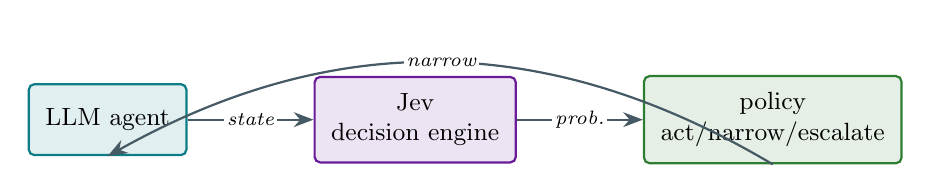
\begin{tikzpicture}
  \node[frontend] (agent) {LLM agent};
  \node[model, right=16mm of agent] (jev) {Jev\\decision engine};
  \node[backend, right=16mm of jev] (policy) {policy\\act/narrow/escalate};
  \draw[flow] (agent) -- node[flowlabel]{state} (jev);
  \draw[flow] (jev) -- node[flowlabel]{prob.} (policy);
  \draw[flow] (policy.south) to[bend right=30] node[flowlabel]{narrow} (agent.south);
\end{tikzpicture}
\vfill
{\large A living companion to \texttt{docs/PLAN.md} and the four research docs.\par}
{\itshape Every figure states where its numbers come from. No illustrative value is a result.\par}
\vspace{1.2cm}
{\large Last built: \today\par}
\end{titlepage}

\tableofcontents
\listoffigures

\chapter*{How to read this book (by goal)}
\addcontentsline{toc}{chapter}{How to read this book (by goal)}
This book teaches everything behind the \texttt{arbiter} project: what Jev is, how
calibration works, how the SDK is designed, and what the evidence says. It is a living
document, rebuilt as the project progresses (see the Build log in Part V).

\section*{Reading paths by goal}

\begin{description}[leftmargin=1.6cm,style=nextline]
  \item[\textcolor{clAccent}{10-minute tour}] Chapter~\ref{ch:building} (what we build) then
    Chapter~\ref{ch:jev} \S\ref{sec:jev-oneline} (what Jev does in one line) then
    Figure~\ref{fig:arch} (the architecture).
  \item[\textcolor{clAccent}{SDK user}] Part~II foundations, then Chapter~\ref{ch:arch}
    (architecture) and Chapter~\ref{ch:decisionpoints} (decision points).
  \item[\textcolor{clAccent}{Researcher}] Chapter~\ref{ch:calibration} (calibration),
    Chapter~\ref{ch:eval} (evaluating agents), and Part~IV (evidence).
  \item[\textcolor{clAccent}{Contributor}] Chapter~\ref{ch:engineering} (engineering
    practices) and the Build log (Part~V).
\end{description}

\section*{Conventions}

Every factual claim carries an evidence label so you always know how much to trust it:
\DOC{} verified in TypeSafe's documentation; \IND{} an independent measurement;
\VENDOR{} a vendor claim; \HYP{} our own hypothesis; \MEAS{} measured by us (with a run
ID). No \MEAS{} labels exist yet, because we have not run experiments.

Every figure and table caption ends with a \textbf{data label} in brackets stating where
its numbers come from: \emph{Illustrative} (a drawing, not data), \emph{Exact} (computed
from a formula), \emph{Reported by \dots} (someone else's measurement, cited), or
\emph{Measured by us}. This rule exists so that a teaching diagram is never mistaken for a
result.

\begin{keyidea}
The whole project rests on one honest distinction: a model's \emph{answer} and its
\emph{calibrated confidence in that answer} are two different things. Most of this book is
about the second one.
\end{keyidea}


\mainmatter

\part{The big picture}
\chapter{What we are building}
\label{ch:building}

We are building \texttt{arbiter} (ARBITER: Agent Runtime for Bounded Inference, Triage,
Evaluation \& Routing): an open-source Python SDK that adds \emph{typed, calibrated
decision points} to an LLM agent a developer already runs (LangChain, Pydantic AI, or the
OpenAI Agents SDK).

\section{The problem in one paragraph}

An LLM agent makes many small, bounded decisions on every loop: which tool to call next,
whether the task is finished, whether it is stuck. Today the same expensive model that
plans and writes text also makes these decisions. That is slow, costly, and, worst of all,
the decision comes back as plain text with \emph{no usable number} telling you how sure the
model is. You cannot tell a confident choice from a coin flip.

\section{The idea}

At each decision point the SDK does four things (Figure~\ref{fig:value}):

\begin{enumerate}[itemsep=2pt]
  \item Build a small, token-budgeted \term{projection} of the agent's state.
  \item Ask a cheap, swappable \term{engine} (Jev by default) a bounded typed question
        and get back \emph{probabilities}.
  \item A deterministic \term{policy} reads the (recalibrated) probability and either
        \textbf{acts}, \textbf{narrows} the LLM's options, or \textbf{escalates} to the
        LLM or a human.
  \item Log the decision and its outcome so thresholds can be fitted and results reproduced.
\end{enumerate}

\begin{figure}[t]\centering
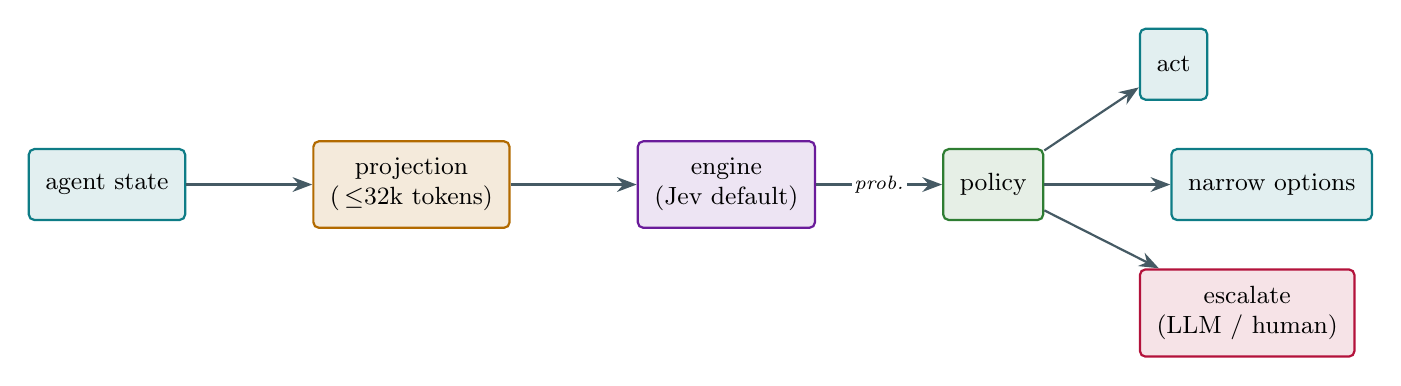
\begin{tikzpicture}[node distance=8mm and 16mm]
  \node[frontend] (state) {agent state};
  \node[infra, right=of state] (proj) {projection\\(\,$\le$32k tokens)};
  \node[model, right=of proj] (engine) {engine\\(Jev default)};
  \node[backend, right=of engine] (policy) {policy};
  \node[frontend, above right=6mm and 12mm of policy] (act) {act};
  \node[frontend, right=of policy] (narrow) {narrow options};
  \node[security, below right=6mm and 12mm of policy] (esc) {escalate\\(LLM / human)};
  \draw[flow] (state) -- (proj);
  \draw[flow] (proj) -- (engine);
  \draw[flow] (engine) -- node[flowlabel]{prob.} (policy);
  \draw[flow] (policy) -- (act);
  \draw[flow] (policy) -- (narrow);
  \draw[flow] (policy) -- (esc);
\end{tikzpicture}
\caption{The arbiter value loop: state becomes a small projection, a cheap engine
returns probabilities, and a deterministic policy acts, narrows, or escalates.\datalabel{Illustrative}}
\label{fig:value}
\end{figure}

\section{Why this and not something else}

The research phase (Part~IV) reached a clear verdict: integrations already exist
(LangChain, Pydantic AI, and Vercel all ship Jev support, and about 200 community projects
exist~\citep{langchain_typesafe,pydantic_typesafe}). What nobody has published is
\emph{controlled evidence}, with proper baselines and trajectory-level calibration, that
inserting a calibrated decision component actually lowers cost per successful task without
hurting reliability. So the project has two co-equal deliverables:

\begin{description}[leftmargin=1.4cm,style=nextline]
  \item[Deliverable A --- the SDK] the instrument developers install.
  \item[Deliverable B --- the evidence] a pre-registered, reproducible study (with a
    released decision dataset and trajectory-checkpoint calibration) that no one else has.
\end{description}

\begin{whyhere}
The engine is \emph{swappable} on purpose. If Jev turns out not to help on your workload,
you change one line to an LLM-backed engine, a small trained classifier, or the
open-weights Laya model~\citep{laya}, and the SDK still works. The product survives a
negative result about any single engine.
\end{whyhere}

\section{What it is not}

It is not a new agent framework (that is an explicit non-goal). It does not plan, write
tool arguments, or generate text; the LLM keeps those jobs. It is never the security or
authorization boundary; deterministic code owns that. The MVP is deliberately small: two
decision points (which tool, and done/stuck) on one host framework.

\begin{checkbox}
Why can a model's answer be right while its confidence is untrustworthy? What would you
measure to catch that? (Answer in Appendix~\ref{app:answers}.)
\end{checkbox}

\chapter{The roadmap}
\label{ch:roadmap}

The project is a sequence of milestones \texttt{M0}--\texttt{M8}, each mapped to a phase of
the research roadmap and separated by \term{gates} (go/modify/stop checkpoints). The rule
is \emph{evidence before claims}: no milestone publishes a cost or reliability number
before the gate that produced it.

\section{Milestones and gates}

\begin{figure}[h]\centering
\fitfig{%
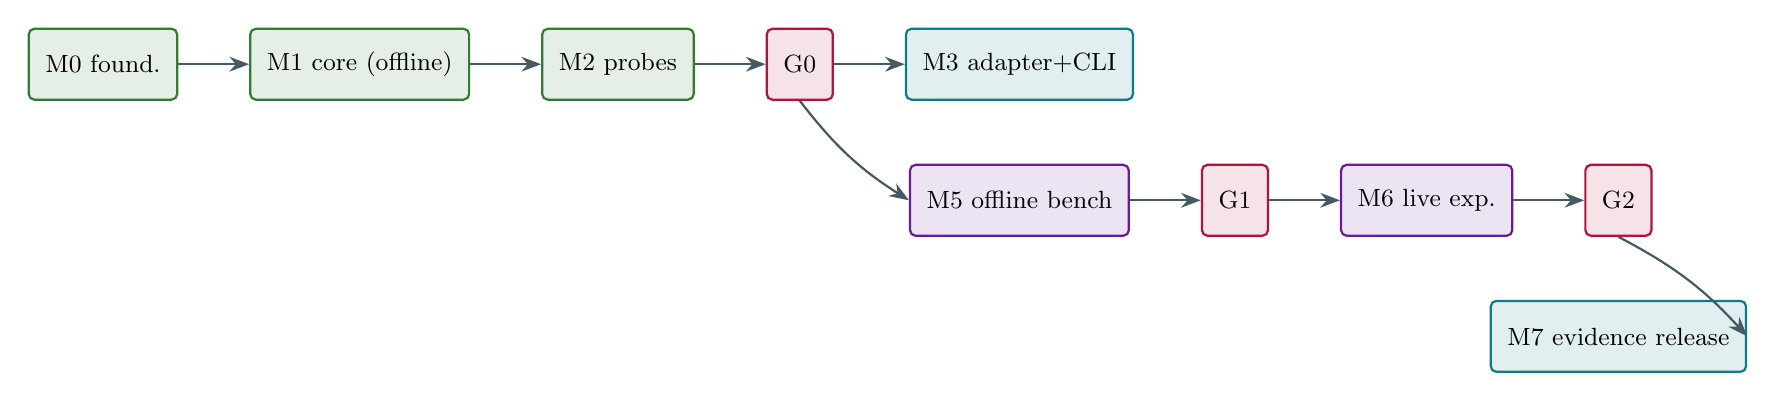
\begin{tikzpicture}[node distance=6mm and 9mm, every node/.style={font=\scriptsize}]
  \node[backend] (m0) {M0 found.};
  \node[backend, right=of m0] (m1) {M1 core (offline)};
  \node[backend, right=of m1] (m2) {M2 probes};
  \node[security, right=of m2] (g0) {G0};
  \node[frontend, right=of g0] (m3) {M3 adapter+CLI};
  \node[model, below=8mm of m3] (m5) {M5 offline bench};
  \node[security, right=of m5] (g1) {G1};
  \node[model, right=of g1] (m6) {M6 live exp.};
  \node[security, right=of m6] (g2) {G2};
  \node[frontend, below=8mm of g2] (m7) {M7 evidence release};
  \draw[flow] (m0)--(m1); \draw[flow] (m1)--(m2); \draw[flow] (m2)--(g0);
  \draw[flow] (g0)--(m3); \draw[flow] (g0.south) to[bend right=10] (m5.west);
  \draw[flow] (m5)--(g1); \draw[flow] (g1)--(m6); \draw[flow] (m6)--(g2);
  \draw[flow] (g2.south) to[bend left=10] (m7.east);
\end{tikzpicture}}
\caption{Milestone flow. Gates G0/G1/G2 are go/modify/stop checkpoints. Product surface
(M3) and evidence (M5/M6) both start after G0.\datalabel{Illustrative}}
\label{fig:milestones}
\end{figure}

\begin{table}[h]\centering\small
\begin{tabular}{@{}llp{5.4cm}@{}}
\toprule
Milestone & Maps to & Ends with \\
\midrule
M0 Foundations & (setup) & this session's docs \\
M1 Core SDK (offline) & research P0/P1 eng. & green offline tests, no keys \\
M2 Engines + probes & research P0 & \textbf{Gate G0} \\
M3 Adapter + CLI & (product) & quickstart under 5 min from cache \\
M4 Public alpha & (product, optional) & v0.1, no claims \\
M5 Offline benchmark & research P1 & \textbf{Gate G1} \\
M6 Live experiment & research P2 & \textbf{Gate G2} \\
M7 Evidence release & write-up & reproducible results page \\
M8 Extensions & research P3 & (optional) \\
\bottomrule
\end{tabular}
\caption{Milestones mapped to the frozen research phases.\datalabel{Reported by docs/PLAN.md \S6}}
\label{tab:milestones}
\end{table}

\section{Estimated timeline}

Dates are estimates, re-planned at each gate. Most of the calendar is API runs, human
labeling, and gate reviews, not coding.

\begin{figure}[h]\centering
\begin{ganttchart}[
  hgrid, vgrid, bar height=0.5, y unit chart=6mm, x unit=3.2mm,
  title height=1, bar/.append style={fill=clBackend!40, draw=clBackend},
  milestone/.append style={fill=clSecurity, draw=clSecurity},
  bar label font=\scriptsize, milestone label font=\scriptsize\itshape,
  title label font=\scriptsize]{1}{30}
  \gantttitle{Weeks from 2026-09-28}{30}\\
  \ganttbar{M0}{1}{1}\\
  \ganttbar{M1}{2}{5}\\
  \ganttbar{M2}{6}{9}\\
  \ganttmilestone{G0}{9}\\
  \ganttbar{M3}{10}{12}\\
  \ganttbar{M5}{10}{17}\\
  \ganttmilestone{G1}{17}\\
  \ganttbar{M6}{18}{25}\\
  \ganttmilestone{G2}{25}\\
  \ganttbar{M7}{26}{28}
\end{ganttchart}
\caption{Estimated schedule to the M7 evidence release (about 20--30 weeks).\datalabel{Illustrative (estimate, docs/PLAN.md \S6.2)}}
\label{fig:gantt}
\end{figure}

\section{How the pieces depend on each other}

Build the thing with the fewest dependencies first. The offline core (log, cache,
projections, policy, calibrators) needs no API keys, so it is built and tested before any
engine that calls a network service.

\begin{figure}[h]\centering
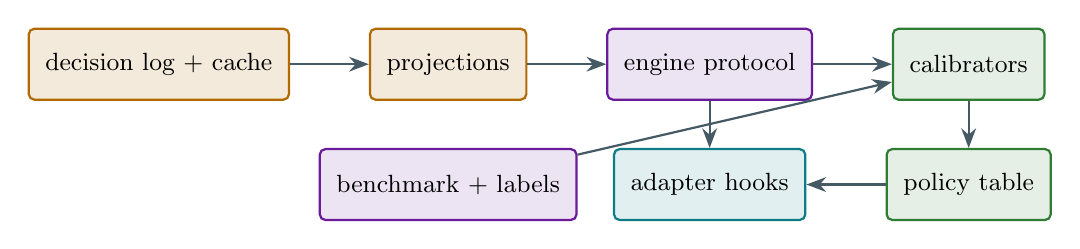
\begin{tikzpicture}[node distance=5mm and 10mm, every node/.style={font=\scriptsize}]
  \node[infra] (log) {decision log + cache};
  \node[infra, right=of log] (proj) {projections};
  \node[model, right=of proj] (eng) {engine protocol};
  \node[backend, right=of eng] (cal) {calibrators};
  \node[backend, below=6mm of cal] (pol) {policy table};
  \node[frontend, below=6mm of eng] (rt) {adapter hooks};
  \node[model, below=6mm of proj] (bench) {benchmark + labels};
  \draw[flow] (log)--(proj); \draw[flow] (proj)--(eng); \draw[flow] (eng)--(cal);
  \draw[flow] (cal)--(pol); \draw[flow] (pol)--(rt); \draw[flow] (eng)--(rt);
  \draw[flow] (bench)--(cal);
\end{tikzpicture}
\caption{Dependency graph: arrows point from a component to what it enables. Offline
components (left) come before networked engines.\datalabel{Illustrative (docs/IMPLEMENTATION\_PLAN.md \S2)}}
\label{fig:deps}
\end{figure}

\begin{checkbox}
Why build the record/replay cache before any real engine? What does it buy you at gate
review time? (Appendix~\ref{app:answers}.)
\end{checkbox}


\part{Foundations}
\chapter{LLM agents and tool calling}
\label{ch:agents}

An \term{LLM agent} is a loop: the model observes state, decides on an action (usually a
tool call), the runtime executes it, and the observation feeds back in. Everything the
decision layer does hangs off this loop, so it is worth being precise about it.

\section{The agent loop}

\begin{figure}[h]\centering
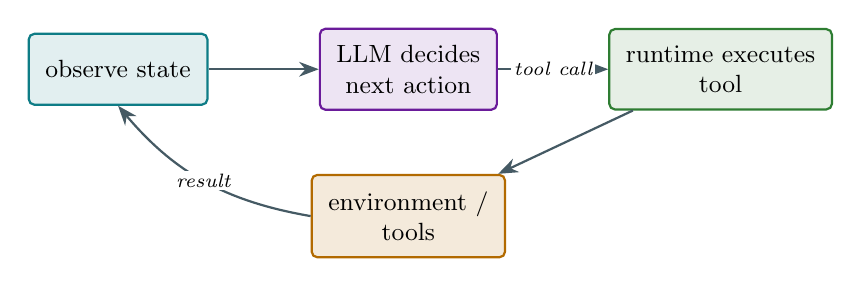
\begin{tikzpicture}[node distance=7mm and 14mm]
  \node[frontend] (obs) {observe state};
  \node[model, right=of obs] (decide) {LLM decides\\next action};
  \node[backend, right=of decide] (exec) {runtime executes\\tool};
  \node[infra, below=8mm of decide] (env) {environment /\\tools};
  \draw[flow] (obs) -- (decide);
  \draw[flow] (decide) -- node[flowlabel]{tool call} (exec);
  \draw[flow] (exec) -- (env);
  \draw[flow] (env.west) to[bend left=20] node[flowlabel]{result} (obs.south);
\end{tikzpicture}
\caption{The agent loop. The decision layer intercepts the ``LLM decides'' step for
bounded, closed-set decisions.\datalabel{Illustrative}}
\label{fig:agentloop}
\end{figure}

\section{Tool calling guarantees shape, not confidence}

Modern APIs let the model emit a structured \term{tool call} (a function name plus JSON
arguments). Structured outputs and strict tool use guarantee the \emph{shape} is valid, but
hosted APIs generally do not return a probability distribution over \emph{which} tool was
chosen. That missing distribution is exactly the primitive the decision layer supplies.

\begin{keyidea}
Frameworks already expose a ``pre-action'' seam: a callable that returns an enum
(allow/deny/ask) or a node name. Escalation there is a boolean, never a probability. The
decision layer plugs into that seam and makes the signal a calibrated probability instead.
\end{keyidea}

\section{Where decisions live at scale}

When a catalog has dozens or hundreds of tools, accuracy degrades: vendors themselves note
tool selection gets worse past roughly 30--50 tools, which is why they ship tool-search and
allowed-tools features. Narrowing the catalog \emph{before} the LLM chooses is a real job,
and a cheap classifier is a natural fit for it. That is decision point DP2, the MVP's first
target (Chapter~\ref{ch:decisionpoints}).

\begin{pitfall}
A tempting shortcut is to let the model both narrow and choose in one call. That reintroduces
the cost you were trying to avoid and hides the decision inside free text, where you cannot
attach a confidence or test it. Keep the bounded decision separate and typed.
\end{pitfall}

\begin{checkbox}
Name two things a hosted tool-calling API guarantees and one thing it does not. Which of the
three does the decision layer add? (Appendix~\ref{app:answers}.)
\end{checkbox}

\chapter{Jev and ``System One'' models}
\label{ch:jev}

\section{What Jev does, in one line}
\label{sec:jev-oneline}

Jev reads a text or JSON \term{state} and answers typed, closed questions about it,
returning probabilities and (for two of the three question types) a confidence
statistic. It does not generate text.\DOC{}~\citep{typesafe_systemone}

TypeSafe calls it a \term{System One} model, after Kahneman's fast, intuitive ``System~1'':
it makes quick bounded judgments, not deliberate multi-step reasoning.

\section{The three primitives}

\begin{figure}[h]\centering
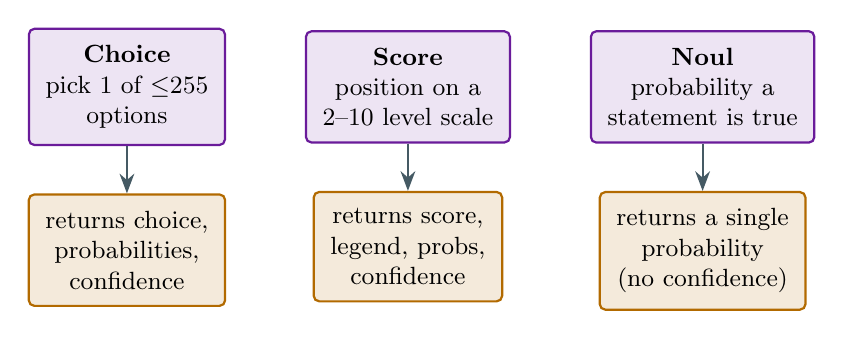
\begin{tikzpicture}[node distance=5mm and 10mm, every node/.style={font=\scriptsize}]
  \node[model] (choice) {\textbf{Choice}\\pick 1 of $\le$255\\options};
  \node[model, right=of choice] (score) {\textbf{Score}\\position on a\\2--10 level scale};
  \node[model, right=of score] (noul) {\textbf{Noul}\\probability a\\statement is true};
  \node[infra, below=6mm of choice] (c2) {returns choice,\\probabilities,\\confidence};
  \node[infra, below=6mm of score] (s2) {returns score,\\legend, probs,\\confidence};
  \node[infra, below=6mm of noul] (n2) {returns a single\\probability\\(no confidence)};
  \draw[flow] (choice)--(c2); \draw[flow] (score)--(s2); \draw[flow] (noul)--(n2);
\end{tikzpicture}
\caption{The three Jev primitives and what each returns.\datalabel{Reported by TypeSafe docs}~\citep{typesafe_primitives}}
\label{fig:primitives}
\end{figure}

\begin{description}[leftmargin=1.4cm,style=nextline]
  \item[Choice] one of up to 255 unordered options; returns the pick, a probability per
    option, and a confidence.\DOC{}
  \item[Score] a position on an ordered 2--10 level scale; the score is a
    probability-weighted mean of level numbers. Numerical interpolation is weakly
    calibrated, so use scores for thresholds, not arithmetic.\DOC{}
  \item[Noul] the probability that a statement is true; no separate confidence field.\DOC{}
\end{description}

\section{Anatomy of a request and response}

You send one \emph{state} and a set of independent \emph{questions}; they are evaluated in
parallel and cannot see each other's answers.\DOC{} Dependent questions need a second
request.

\begin{lstlisting}[language=jsonc,caption={A Choice request and its response (schematic).},label={lst:jevreq}]
// request
{ "state": { "task": "book a flight", "last_actions": ["search_flights"] },
  "model": "jev-1.13.0",
  "questions": [ { "id": "next_tool", "type": "choice",
                   "options": ["select_seat","pay","search_flights","none_of_the_above"] } ] }
// response
{ "answers": { "next_tool": { "choice": "select_seat",
      "probabilities": {"select_seat":0.71,"pay":0.20,"search_flights":0.08,
                        "none_of_the_above":0.01},
      "confidence": 0.68 } },
  "model": "jev-1.13.0", "usage": {"input_tokens": 41} }
\end{lstlisting}

\begin{worked}
Cost is dominated by input tokens: at the list price of \$0.042 per million input tokens
with free output, 20{,}000 decisions of about 1{,}500 input tokens each cost roughly
\$1.26.\DOC{}~\citep{typesafe_models} The limits that shape the SDK: at most 255 Choice
options, 2--10 Score levels, and 64k tokens per request (32k for state plus the longest
question).\DOC{}
\end{worked}

\section{The nine documented failure modes}

TypeSafe publishes a ``jaggedness'' page listing where Jev fails and how to work around
it.\DOC{}~\citep{typesafe_jaggedness} These are load-bearing for the design.

\begin{figure}[h]\centering
\small
\begin{tabular}{@{}p{4.6cm}p{7.4cm}@{}}
\toprule
Failure mode & Consequence for the design \\
\midrule
1. Literal reading & Question wording becomes a versioned artifact. \\
2. Math / counting & Keep arithmetic and counts in code. \\
3. Date/time comparison & Extract components; compute dates in code. \\
4. Indirection / multi-hop & Excludes planning-level decisions. \\
5. Large irrelevant state & Send projections, never full history. \\
6. Adversarial content & Cannot be the security boundary. \\
7. Contradictory criteria & Criteria design discipline. \\
8. No cross-primitive invariants & Do not transfer thresholds between primitives. \\
9. No generation & The LLM writes all text and arguments. \\
\bottomrule
\end{tabular}
\caption{The nine documented failure modes and what each forces in the architecture.\datalabel{Reported by TypeSafe docs}~\citep{typesafe_jaggedness}}
\label{fig:failuremodes}
\end{figure}

\begin{whyhere}
Every one of these nine drives a concrete rule later: projections (mode~5), deterministic
verifiers (modes~2--3), advisory-only authority (mode~6), frozen question wording
(mode~1), and per-primitive thresholds (mode~8). The design is essentially a disciplined
response to this table.
\end{whyhere}

\begin{checkbox}
Jev returns a probability of \(0.99\) that a shell command is safe. Give two reasons from
this chapter why code, not Jev, must still decide whether to run it. (Appendix~\ref{app:answers}.)
\end{checkbox}

\chapter{Probability, confidence, and calibration}
\label{ch:calibration}

This is the conceptual center of the project. A model can be accurate yet
\emph{miscalibrated}: its stated probabilities do not match how often it is right. Gating
actions on an untrustworthy probability is worse than not gating at all.

\section{Calibration, defined}

A model is \term{calibrated} if, among all the times it says ``0.8'', it is right about
80\% of the time. This is a property of \emph{groups} of predictions, not any single one.
TypeSafe states calibration exactly this way and warns it ``is not a guarantee about any
single answer.''\DOC{}

\begin{figure}[h]\centering
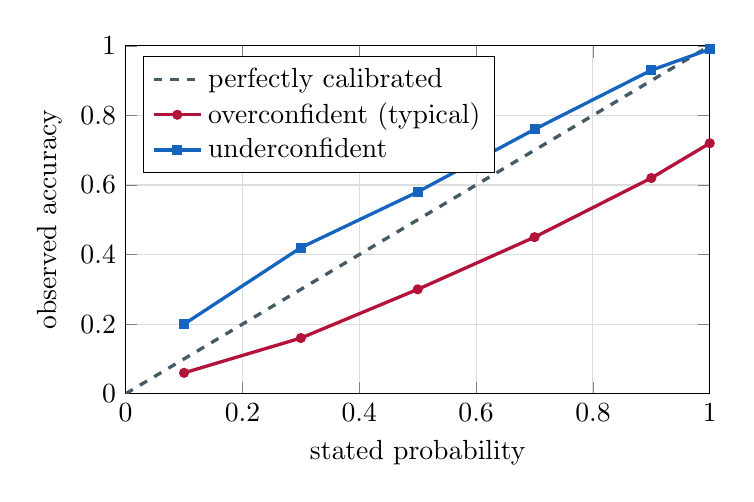
\begin{tikzpicture}
\begin{axis}[width=9cm,height=6cm,xlabel={stated probability},ylabel={observed accuracy},
  xmin=0,xmax=1,ymin=0,ymax=1,legend pos=north west,legend cell align=left,
  grid=both, grid style={clExternal!20}]
  \addplot[very thick, clExternal, dashed] coordinates {(0,0)(1,1)};
  \addlegendentry{perfectly calibrated}
  \addplot[very thick, clSecurity, mark=*, mark size=1.2] coordinates
    {(0.1,0.06)(0.3,0.16)(0.5,0.30)(0.7,0.45)(0.9,0.62)(1.0,0.72)};
  \addlegendentry{overconfident (typical)}
  \addplot[very thick, clAccent, mark=square*, mark size=1.2] coordinates
    {(0.1,0.20)(0.3,0.42)(0.5,0.58)(0.7,0.76)(0.9,0.93)(1.0,0.99)};
  \addlegendentry{underconfident}
\end{axis}
\end{tikzpicture}
\caption{A reliability diagram. Points on the dashed line are calibrated; below it is
overconfident, above it is underconfident.\datalabel{Illustrative (synthetic data)}}
\label{fig:reliability}
\end{figure}

\section{Measuring miscalibration: ECE and the noise floor}

The \term{Expected Calibration Error (ECE)} bins predictions by stated probability and
averages the gap between confidence and accuracy in each bin, weighted by bin size:
\[
\mathrm{ECE} = \sum_{b=1}^{B} \frac{n_b}{N}\,\bigl|\,\mathrm{acc}(b) - \mathrm{conf}(b)\,\bigr|.
\]
A subtlety that honest evaluations respect: with finite samples, even a perfectly calibrated
model shows a small nonzero ECE. That is the \term{noise floor}. Reporting ECE without its
floor overstates miscalibration.

\begin{figure}[h]\centering
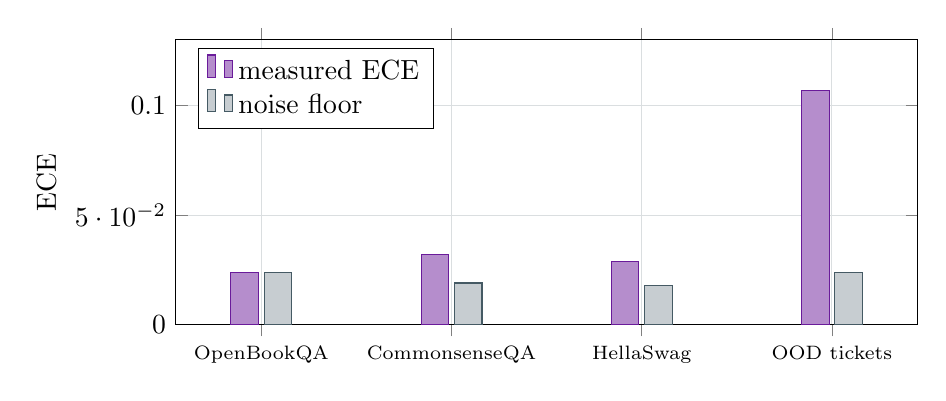
\begin{tikzpicture}
\begin{axis}[width=11cm,height=5.2cm,ybar,bar width=10pt,
  symbolic x coords={OpenBookQA,CommonsenseQA,HellaSwag,OOD tickets},
  xtick=data, x tick label style={font=\scriptsize},
  ylabel={ECE}, ymin=0, ymax=0.13, legend pos=north west, legend cell align=left,
  enlarge x limits=0.15, grid=both, grid style={clExternal!20}]
  \addplot[fill=clModel!50, draw=clModel] coordinates
    {(OpenBookQA,0.024)(CommonsenseQA,0.032)(HellaSwag,0.029)(OOD tickets,0.107)};
  \addlegendentry{measured ECE}
  \addplot[fill=clExternal!30, draw=clExternal] coordinates
    {(OpenBookQA,0.024)(CommonsenseQA,0.019)(HellaSwag,0.018)(OOD tickets,0.024)};
  \addlegendentry{noise floor}
\end{axis}
\end{tikzpicture}
\caption{Jev's ECE is near the noise floor in distribution but about 4.4\(\times\) the floor
out of distribution.\datalabel{Reported by jev-ood-calibration}~\citep{jev_ood_calibration}}
\label{fig:ece}
\end{figure}

\section{Risk--coverage: the operating decision}

Gating is a trade: act only when confident (high \term{coverage} costs accuracy; low
coverage buys it). A \term{risk--coverage curve} shows accuracy on the automated fraction as
you sweep the threshold. The product's G0 gate asks for coverage $\ge 50\%$ at a chosen
precision target.

\begin{figure}[h]\centering
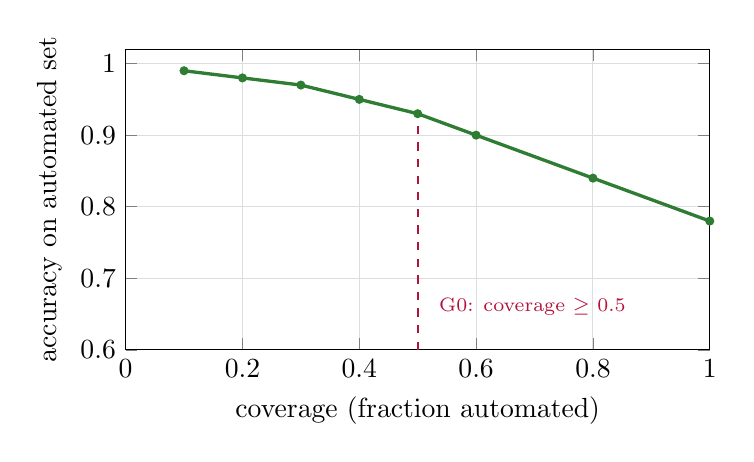
\begin{tikzpicture}
\begin{axis}[width=9cm,height=5.4cm,xlabel={coverage (fraction automated)},
  ylabel={accuracy on automated set}, xmin=0,xmax=1,ymin=0.6,ymax=1.02,
  grid=both, grid style={clExternal!20}]
  \addplot[very thick, clBackend, mark=*, mark size=1] coordinates
    {(0.1,0.99)(0.2,0.98)(0.3,0.97)(0.4,0.95)(0.5,0.93)(0.6,0.90)(0.8,0.84)(1.0,0.78)};
  \draw[clSecurity, dashed, thick] (axis cs:0.5,0.6) -- (axis cs:0.5,0.93);
  \node[clSecurity, font=\scriptsize, anchor=west] at (axis cs:0.52,0.66) {G0: coverage $\ge$ 0.5};
\end{axis}
\end{tikzpicture}
\caption{A risk--coverage curve: acting only on the most confident decisions raises
accuracy on the automated fraction.\datalabel{Illustrative (synthetic data)}}
\label{fig:riskcov}
\end{figure}

\section{Fixing calibration after the fact}

Two standard post-hoc recalibrators, fitted on a held-out labeled split:

\begin{description}[leftmargin=1.4cm,style=nextline]
  \item[Temperature scaling] divide the logits by a single learned scalar $T$ before the
    softmax~\citep{guo_calibration}. Simple, but it needs \emph{logits}. If the API returns
    only probabilities, or a probability is exactly 1.0, temperature scaling is undefined
    (\(\log 1 = 0\) after the softmax, \(\log\) of a saturated prob is problematic). This is
    a real constraint for Jev (see the pitfall).
  \item[Isotonic regression] fit a monotonic step function from stated probability to
    observed frequency. Works on probabilities directly and handled Jev well in an
    independent study, reaching ECE $\approx 0.01$ with a few hundred labels~\citep{jev_calibration_anthus}.
\end{description}

\begin{figure}[h]\centering
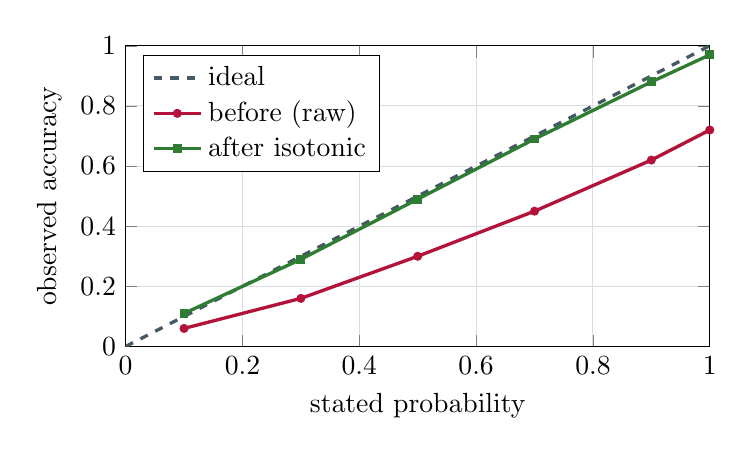
\begin{tikzpicture}
\begin{axis}[width=9cm,height=5.4cm,xlabel={stated probability},ylabel={observed accuracy},
  xmin=0,xmax=1,ymin=0,ymax=1,legend pos=north west,legend cell align=left,
  grid=both, grid style={clExternal!20}]
  \addplot[very thick, clExternal, dashed] coordinates {(0,0)(1,1)};
  \addlegendentry{ideal}
  \addplot[very thick, clSecurity, mark=*, mark size=1] coordinates
    {(0.1,0.06)(0.3,0.16)(0.5,0.30)(0.7,0.45)(0.9,0.62)(1.0,0.72)};
  \addlegendentry{before (raw)}
  \addplot[very thick, clBackend, mark=square*, mark size=1] coordinates
    {(0.1,0.11)(0.3,0.29)(0.5,0.49)(0.7,0.69)(0.9,0.88)(1.0,0.97)};
  \addlegendentry{after isotonic}
\end{axis}
\end{tikzpicture}
\caption{Post-hoc recalibration pulls an overconfident model toward the diagonal.\datalabel{Illustrative (synthetic data), effect direction reported by Jev-Calibration}~\citep{jev_calibration_anthus}}
\label{fig:recal}
\end{figure}

\begin{pitfall}
Independent testers found Jev returns probability \emph{exactly} 1.0 on many items, some of
them wrong~\citep{jev_baselines_eval}. A saturated 1.0 breaks temperature scaling and
collapses isotonic bins. The SDK's rule: verify whether logits are available; if not, use
isotonic or histogram binning with epsilon-clipping, and add a ``saturated'' band that
\emph{always escalates} for any authority above a plain filter. ``1.0 is not proof.''
\end{pitfall}

\begin{whyhere}
Independent studies also found the vendor \texttt{confidence} field was \emph{less}
calibrated than the maximum option probability~\citep{jev_ood_calibration}. So the SDK
defaults to gating on max probability, logs both, and lets the G0 study pick the winner.
Thresholds are fitted per decision point, per primitive, per model version, and refit when
wording, catalog, or version changes.
\end{whyhere}

\section{Conformal prediction (a brief note)}

\term{Conformal prediction} builds a set of options guaranteed (under exchangeability) to
contain the truth with a chosen probability, using a calibration set. Robotics work
(KnowNo) used it to decide when an agent should ask for help~\citep{knowno}. It is a natural
future tool for the escalation policy; the MVP starts with simpler threshold gating.

\begin{checkbox}
A model scores 92\% accuracy and ECE 0.15. Your policy acts whenever confidence
$\ge 0.9$. Why might this be dangerous, and which figure in this chapter would you inspect
first? (Appendix~\ref{app:answers}.)
\end{checkbox}

\chapter{Routers, cascades, and verifiers}
\label{ch:routers}

The decision layer sits in a long line of ideas for spending less compute without losing
quality. Knowing where they succeed, and where they usually fail, keeps our claims honest.

\section{Routers}

A \term{router} sends each query to the cheapest model likely to handle it. RouteLLM trains
strong-vs-weak routers from preference data and reports large savings at matched
quality~\citep{routellm}. The cautionary result: benchmarks found many routers barely beat a
trivial ``mix models at random in the right proportion'' baseline, and routers trained on
one distribution were near-random on another. Baselines matter.

\section{Cascades}

A \term{cascade} tries a cheap model first and escalates to an expensive one when a
reliability score is low. FrugalGPT is the canonical example~\citep{frugalgpt}. But theory
shows confidence-based deferral \emph{provably fails} when the downstream model is a
specialist, under label noise, and under distribution shift~\citep{cascade_deferral}.

\begin{figure}[h]\centering
\fitfig{%
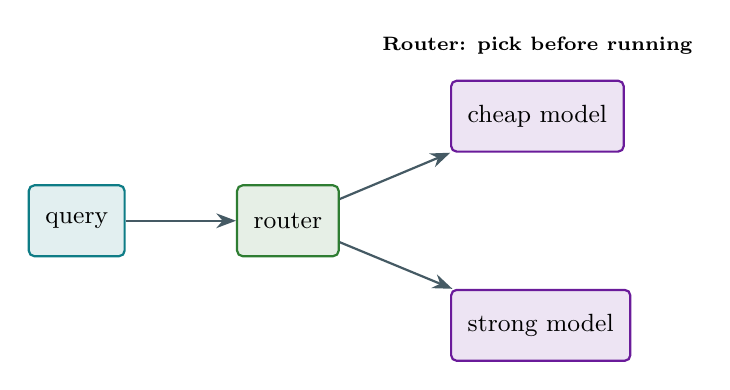
\begin{tikzpicture}[node distance=6mm and 14mm, every node/.style={font=\scriptsize}]
  % router (top)
  \node[frontend] (q1) {query};
  \node[backend, right=of q1] (r) {router};
  \node[model, above right=4mm and 14mm of r] (weak) {cheap model};
  \node[model, below right=4mm and 14mm of r] (strong) {strong model};
  \draw[flow] (q1)--(r); \draw[flow] (r)--(weak); \draw[flow] (r)--(strong);
  \node[font=\scriptsize\bfseries, above=2mm of weak] {Router: pick before running};
\end{tikzpicture}}
\par\vspace{6mm}
\fitfig{%
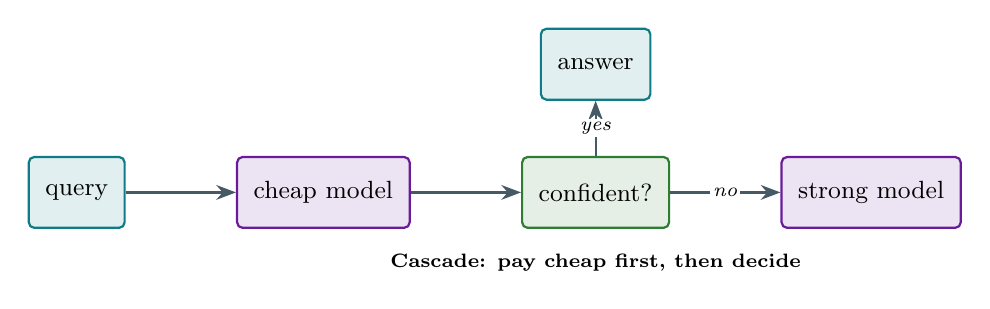
\begin{tikzpicture}[node distance=6mm and 14mm, every node/.style={font=\scriptsize}]
  % cascade (separate picture, well below)
  \node[frontend] (q2) {query};
  \node[model, right=of q2] (cheap) {cheap model};
  \node[backend, right=of cheap] (gate) {confident?};
  \node[model, right=of gate] (exp) {strong model};
  \node[frontend, above=7mm of gate] (out) {answer};
  \draw[flow] (q2)--(cheap); \draw[flow] (cheap)--(gate);
  \draw[flow] (gate)-- node[flowlabel]{yes} (out);
  \draw[flow] (gate)-- node[flowlabel]{no} (exp);
  \node[font=\scriptsize\bfseries, below=2mm of gate] {Cascade: pay cheap first, then decide};
\end{tikzpicture}}
\caption{Router vs cascade. A router decides \emph{before} paying (top); a cascade pays the
cheap model first, then defers on low confidence (bottom).\datalabel{Illustrative}}
\label{fig:routercascade}
\end{figure}

\begin{keyidea}
Because Jev is so cheap, it acts more like a \emph{pre-generation router} (decide before
paying for the LLM) than a cascade rung. What decides whether it helps is not its latency
but its \emph{error rate on the specific decision}, and whether its confidence is calibrated
enough to gate on.
\end{keyidea}

\section{Verifiers and the ``information the proposer lacks'' rule}

Separating a \term{proposer} (the LLM) from a \term{scorer/verifier} helps in robotics and
web agents, but the literature is consistent about \emph{why}: it helps when the scorer has
information the proposer does not, such as execution results or environment state, not merely
because it is a second model. Imperfect verifiers also cap the gains and can be gamed at
large sample counts.

\begin{whyhere}
This sets our expectation for the honest outcome: ``cheaper decisions at equal or slightly
lower accuracy,'' not ``a strictly better agent.'' The evaluation is designed to detect
exactly that, and the arms (Chapter~\ref{ch:eval}) separate ``typed decision helped'' from
``Jev specifically helped'' from ``more compute helped.''
\end{whyhere}

\begin{checkbox}
Why is a cheap, calibrated classifier better modeled as a pre-generation router than as a
cascade rung? (Appendix~\ref{app:answers}.)
\end{checkbox}

\chapter{Evaluating agents honestly}
\label{ch:eval}

An impressive demo proves nothing. This chapter is the measurement discipline that makes the
project's claims trustworthy, drawn from the agent-evaluation literature.

\section{Reliability: pass@k vs pass\textasciicircum k}

\term{pass@k} asks whether the agent succeeds in \emph{at least one} of $k$ tries; it flatters
flaky agents. \term{pass\^{}k} asks whether it succeeds in \emph{all} $k$ tries; it measures
reliability~\citep{tau_bench}. As $k$ grows the two diverge sharply for an unreliable agent.

\begin{figure}[h]\centering
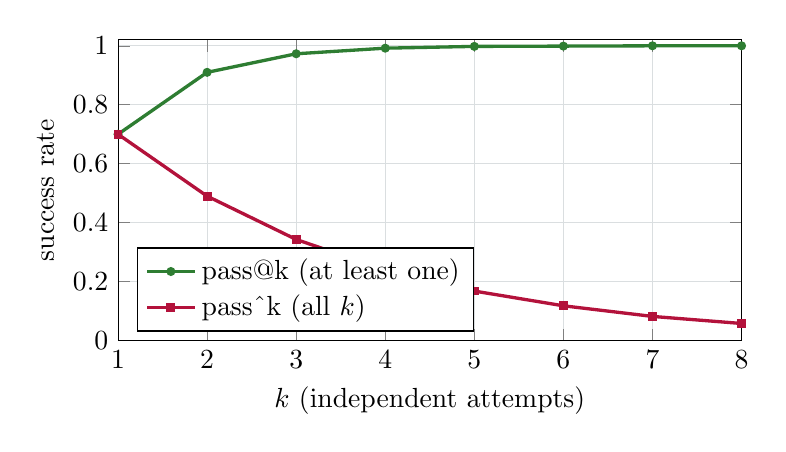
\begin{tikzpicture}
\begin{axis}[width=9.5cm,height=5.4cm,xlabel={$k$ (independent attempts)},ylabel={success rate},
  xmin=1,xmax=8,ymin=0,ymax=1.02,legend pos=south west,legend cell align=left,
  xtick={1,2,3,4,5,6,7,8}, grid=both, grid style={clExternal!20}]
  % per-attempt success p=0.7
  \addplot[very thick, clBackend, mark=*, mark size=1] coordinates
    {(1,0.7)(2,0.91)(3,0.973)(4,0.992)(5,0.998)(6,0.999)(7,1.0)(8,1.0)};
  \addlegendentry{pass@k (at least one)}
  \addplot[very thick, clSecurity, mark=square*, mark size=1] coordinates
    {(1,0.7)(2,0.49)(3,0.343)(4,0.240)(5,0.168)(6,0.118)(7,0.082)(8,0.058)};
  \addlegendentry{pass\^{}k (all $k$)}
\end{axis}
\end{tikzpicture}
\caption{For a per-attempt success of 0.7, pass@k rushes to 1 while pass\textasciicircum k
collapses. Reliability is the honest metric.\datalabel{Exact (computed from $p=0.7$)}}
\label{fig:passk}
\end{figure}

\section{Cost per successful task and the Pareto frontier}

Accuracy alone hides the bill. The right object is the \term{accuracy--cost Pareto frontier}:
plot each system by cost and success, and compare frontiers, not single
points~\citep{ai_agents_that_matter}. A famous result: a plain ``retry'' baseline beat an
elaborate agent at a fraction of the cost, which is why baselines like ARM-A5 (random) and
ARM-A6 (matched compute) exist in our design.

\begin{figure}[h]\centering
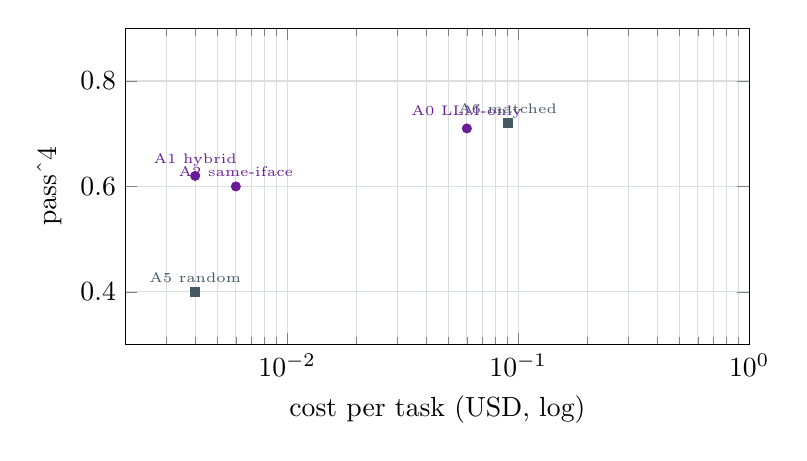
\begin{tikzpicture}
\begin{axis}[width=9.5cm,height=5.6cm,xlabel={cost per task (USD, log)},ylabel={pass\^{}4},
  xmode=log, xmin=0.002,xmax=1,ymin=0.3,ymax=0.9,legend pos=south east,
  legend cell align=left, grid=both, grid style={clExternal!20},
  nodes near coords, point meta=explicit symbolic, every node near coord/.append style={font=\tiny}]
  \addplot[only marks, mark=*, clModel, mark size=1.6] coordinates
    {(0.004,0.62)[A1 hybrid] (0.06,0.71)[A0 LLM-only] (0.006,0.60)[A2 same-iface]};
  \addplot[only marks, mark=square*, clExternal, mark size=1.6] coordinates
    {(0.09,0.72)[A6 matched] (0.004,0.40)[A5 random]};
\end{axis}
\end{tikzpicture}
\caption{Illustrative accuracy--cost plot. The question is whether the hybrid (A1) sits
up-and-left of the baseline (A0) and beats the random control (A5).\datalabel{Illustrative (synthetic data); arm definitions from docs/PLAN.md \S9}}
\label{fig:pareto}
\end{figure}

\section{The controls that stop us fooling ourselves}

\begin{description}[leftmargin=1.4cm,style=nextline]
  \item[Same-interface baseline (ARM-A2)] an LLM answering the \emph{same} typed questions,
    to separate ``typed decision points help'' from ``Jev specifically helps.''
  \item[Matched compute (ARM-A6)] give the baseline the same extra budget the hybrid spends,
    so a win is not just ``more compute.''
  \item[Random policy (ARM-A5)] the same machinery making random decisions, to control for
    the structure of the intervention.
  \item[Oracle (ARM-A4)] perfect decisions, an upper bound: if even the oracle does not help,
    the chosen decision points are not the bottleneck.
  \item[Pre-registration] fix arms, metrics, thresholds, and seeds \emph{before} looking at
    results; fit thresholds on a disjoint split; report bootstrap confidence intervals over
    $\ge 3$ seeds.
\end{description}

\begin{pitfall}
Never use an LLM judge as sole ground truth for accuracy: it measures \emph{agreement}, not
correctness. One study reported 91.5\% agreement with a frontier model, but with no human
labels that is agreement, not accuracy~\citep{good_start_labs}.
\end{pitfall}

\begin{checkbox}
An agent reports pass@8 of 0.95. Why might its pass\^{}8 be under 0.6, and which figure shows
it? (Appendix~\ref{app:answers}.)
\end{checkbox}


\part{The system}
\chapter{Decision points DP1--DP7}
\label{ch:decisionpoints}

The architecture is organized around seven recurring decision points. Each has a natural Jev
primitive, some evidence it can be served, and a \term{risk class} that caps how much
authority the engine may have.

\begin{figure}[h]\centering
\small
\begin{tabular}{@{}llp{5.2cm}l@{}}
\toprule
ID & Decision & Primitive / evidence & Authority \\
\midrule
DP1 & intent / route & Choice; \IND{} within a few pts of a frontier LLM & may act \\
DP2 & \textbf{tool pre-selection} & Choice; \VENDOR{} skill-suggestion cookbook & narrows only \\
DP3 & action risk & Choice/Noul; \IND{} 91.7\% on 60 cases & \textbf{advisory only} \\
DP4 & \textbf{done / stuck} & Noul/Choice; evidence thin & control flow only \\
DP5 & observation triage & Noul per item; \VENDOR{} RAG cookbooks & filter only \\
DP6 & output verification & Choice/Noul; \IND{} agreement not accuracy & routes to review \\
DP7 & escalation & confidence from any DP & control flow \\
\bottomrule
\end{tabular}
\caption{The decision-point taxonomy. The MVP uses DP2 and DP4 (bold); DP3 is shadow-only,
the rest are deferred.\datalabel{Reported by docs/ARCHITECTURE.md \S3}}
\label{fig:dptaxonomy}
\end{figure}

\section{The design rule}

Jev is a candidate only for decisions whose answer space is \emph{closed}, whose relevant
state fits in about 32k tokens, and whose consequences can be bounded by code. Authority
scales inversely with risk.

\begin{figure}[h]\centering
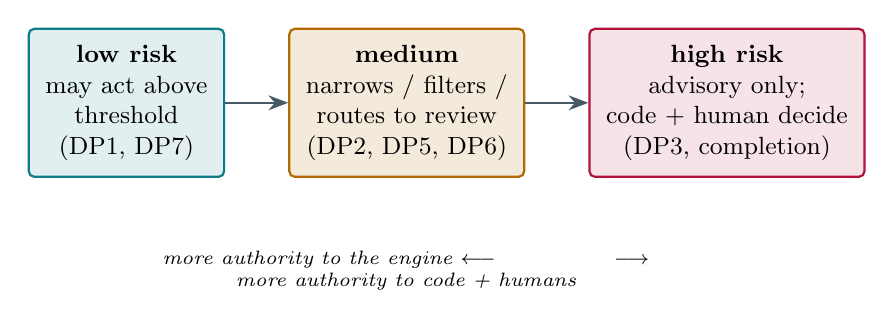
\begin{tikzpicture}[node distance=5mm and 8mm, every node/.style={font=\scriptsize}]
  \node[frontend] (low) {\textbf{low risk}\\may act above\\threshold\\(DP1, DP7)};
  \node[infra, right=of low] (med) {\textbf{medium}\\narrows / filters /\\routes to review\\(DP2, DP5, DP6)};
  \node[security, right=of med] (high) {\textbf{high risk}\\advisory only;\\code + human decide\\(DP3, completion)};
  \draw[flow] (low)--(med); \draw[flow] (med)--(high);
  \node[below=8mm of med, font=\scriptsize\itshape, text width=8.5cm, align=center]
    {more authority to the engine \(\longleftarrow\)\hspace{1.5cm}\(\longrightarrow\) more authority to code + humans};
\end{tikzpicture}
\caption{Authority classes: the riskier the consequence, the less the engine may decide on
its own.\datalabel{Illustrative (docs/ARCHITECTURE.md \S3, \S10)}}
\label{fig:authority}
\end{figure}

\section{The two MVP decisions}

\begin{description}[leftmargin=1.4cm,style=nextline]
  \item[DP2 tool pre-selection] a Choice over the permission-filtered catalog, always with a
    ``\texttt{none\_of\_the\_above}'' escape hatch. High confidence exposes one tool; medium
    exposes the top-$k$; low exposes the full catalog. The LLM still writes the arguments. It
    is advisory: the LLM may pick outside the top-$k$, and the disagreement is logged.
  \item[DP4 done / stuck] a Noul/Choice over a projection of the task, acceptance criteria,
    and the last few actions. ``Done'' with high confidence only \emph{triggers} a
    deterministic completion verifier; it never ends the run by itself. v1 is scoped to
    ``done'' plus loop/repeat detection; ``drift from goal'' waits for an operational
    definition.
\end{description}

\begin{pitfall}
Options are permission-filtered per step, so the option \emph{set} changes every call.
``Fix the option order'' really means ``fix a stable sort key (by tool ID) that is invariant
under filtering.'' Otherwise calibration fitted on one option ordering will not transfer.
\end{pitfall}

\begin{checkbox}
Why does DP2 narrow options rather than pick the final tool, and why does DP4 never declare
success on its own? (Appendix~\ref{app:answers}.)
\end{checkbox}

\chapter{SDK architecture}
\label{ch:arch}

The SDK extends the recommended architecture from the research (LLM-first, engine advisory):
the LLM plans and writes; a swappable engine answers bounded questions; deterministic code
owns safety, permissions, arithmetic, and verification.

\section{Components}

\begin{figure}[t]\centering
\fitfig{%
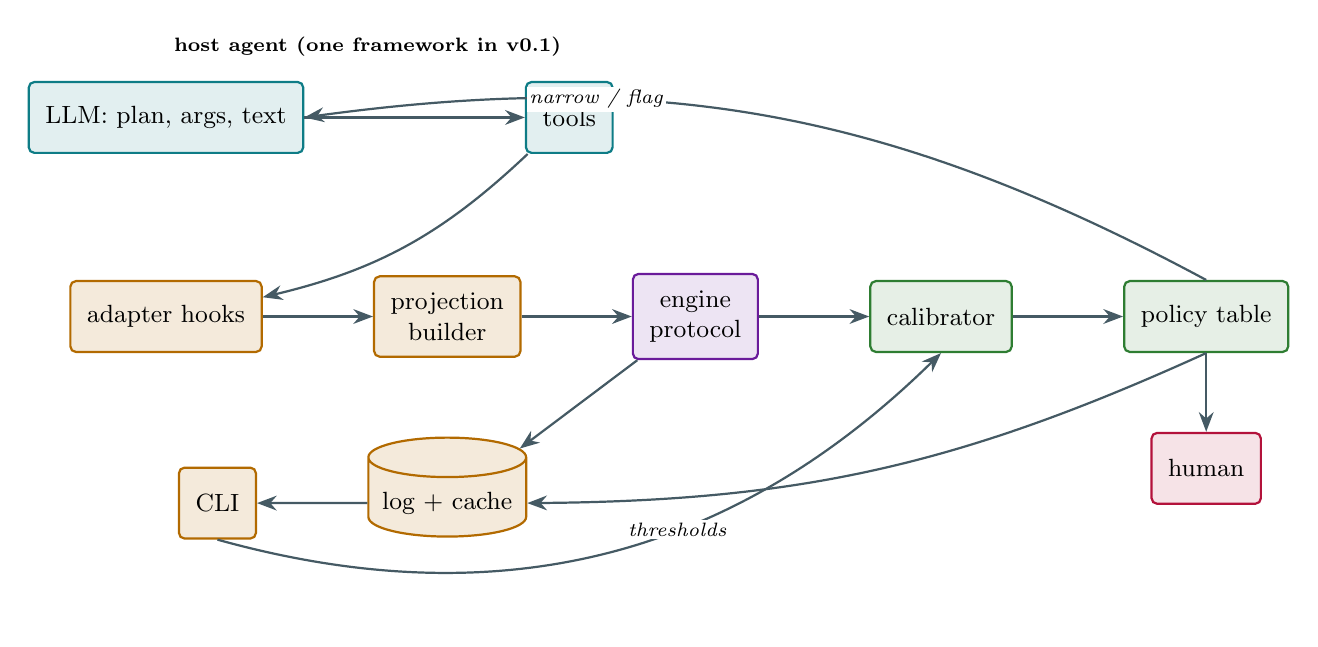
\begin{tikzpicture}[node distance=9mm and 14mm, every node/.style={font=\scriptsize}]
  % Host agent row (top)
  \node[frontend] (llm) {LLM: plan, args, text};
  \node[frontend, right=28mm of llm] (tools) {tools};
  \node[font=\scriptsize\bfseries] at ($(llm)!0.5!(tools)+(0,9mm)$) {host agent (one framework in v0.1)};

  % SDK pipeline row (middle)
  \node[infra, below=16mm of llm] (adapter) {adapter hooks};
  \node[infra, right=of adapter] (proj) {projection\\builder};
  \node[model, right=of proj] (eng) {engine\\protocol};
  \node[backend, right=of eng] (cal) {calibrator};
  \node[backend, right=of cal] (pol) {policy table};

  % SDK support row (bottom)
  \node[store, below=10mm of proj] (log) {log + cache};
  \node[infra, left=14mm of log] (cli) {CLI};
  \node[security, below=10mm of pol] (human) {human};

  % pipeline
  \draw[flow] (adapter)--(proj); \draw[flow] (proj)--(eng);
  \draw[flow] (eng)--(cal); \draw[flow] (cal)--(pol);
  % host <-> sdk
  \draw[flow] (llm)--(tools);
  \draw[flow] (tools) to[bend left=15] (adapter);
  \draw[flow] (pol.north) to[bend right=18] node[flowlabel,pos=0.7]{narrow / flag} (llm.east);
  \draw[flow] (pol)--(human);
  % logging + cli + calibration feedback
  \draw[flow] (eng)--(log); \draw[flow] (pol.south) to[bend left=12] (log.east);
  \draw[flow] (log)--(cli);
  \draw[flow] (cli.south) to[bend right=30] node[flowlabel,pos=0.6]{thresholds} (cal.south);
\end{tikzpicture}}
\caption{SDK components. The engine is advisory; the policy narrows or escalates; code owns
execution and safety.\datalabel{Illustrative (docs/ARCHITECTURE.md \S4, docs/PLAN.md \S4)}}
\label{fig:arch}
\end{figure}

\section{One loop iteration (MVP)}

\begin{figure}[h]\centering
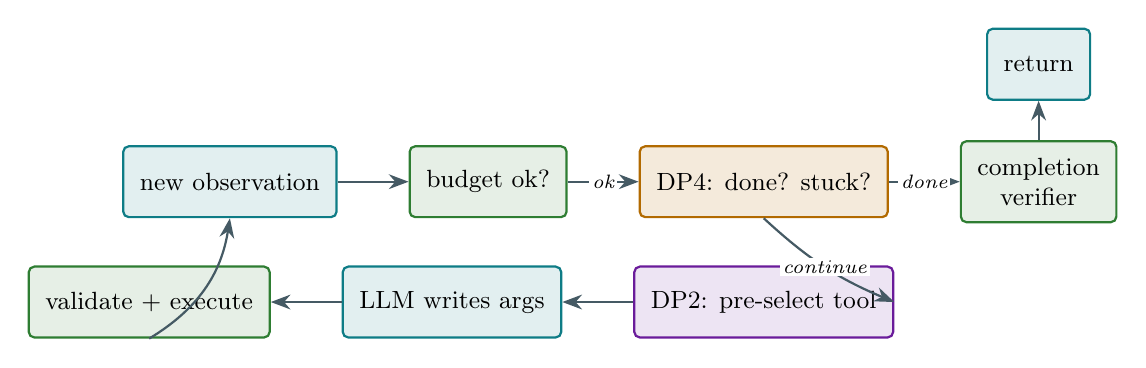
\begin{tikzpicture}[node distance=4.5mm and 9mm, every node/.style={font=\scriptsize}]
  \node[frontend] (obs) {new observation};
  \node[backend, right=of obs] (budget) {budget ok?};
  \node[infra, right=of budget] (dp4) {DP4: done? stuck?};
  \node[backend, right=of dp4] (ver) {completion\\verifier};
  \node[frontend, above=5mm of ver] (done) {return};
  \node[model, below=6mm of dp4] (dp2) {DP2: pre-select tool};
  \node[frontend, left=of dp2] (llm) {LLM writes args};
  \node[backend, left=of llm] (val) {validate + execute};
  \draw[flow] (obs)--(budget); \draw[flow] (budget)-- node[flowlabel]{ok} (dp4);
  \draw[flow] (dp4)-- node[flowlabel]{done} (ver); \draw[flow] (ver)--(done);
  \draw[flow] (dp4.south) to[bend right=10] node[flowlabel]{continue} (dp2.east);
  \draw[flow] (dp2)--(llm); \draw[flow] (llm)--(val);
  \draw[flow] (val.south) to[bend right=25] (obs.south);
\end{tikzpicture}
\caption{The MVP loop: DP4 monitors progress, DP2 narrows the tool, the LLM writes
arguments, and code validates and executes.\datalabel{Illustrative (docs/PLAN.md \S5)}}
\label{fig:loop}
\end{figure}

\section{A single decision, in sequence}

\begin{figure}[h]\centering
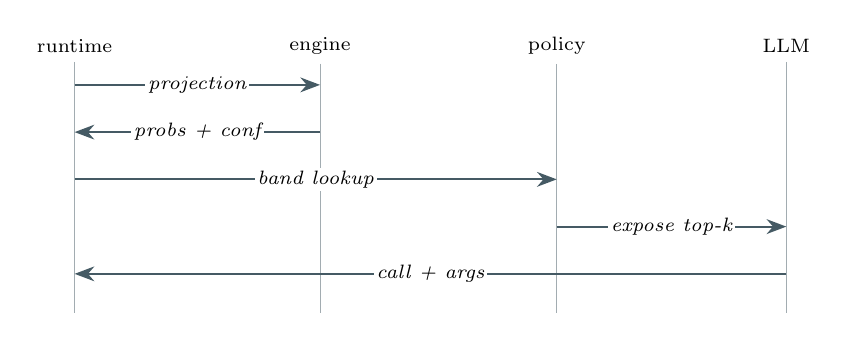
\begin{tikzpicture}[node distance=3mm and 20mm, every node/.style={font=\scriptsize}]
  \node (rt) {runtime};
  \node[right=of rt] (eng) {engine};
  \node[right=of eng] (pol) {policy};
  \node[right=of pol] (llm) {LLM};
  \foreach \n in {rt,eng,pol,llm} { \draw[clExternal!50] (\n) -- ++(0,-3.4); }
  \draw[flow] ($(rt)+(0,-0.5)$) -- node[flowlabel]{projection} ($(eng)+(0,-0.5)$);
  \draw[flow] ($(eng)+(0,-1.1)$) -- node[flowlabel]{probs + conf} ($(rt)+(0,-1.1)$);
  \draw[flow] ($(rt)+(0,-1.7)$) -- node[flowlabel]{band lookup} ($(pol)+(0,-1.7)$);
  \draw[flow] ($(pol)+(0,-2.3)$) -- node[flowlabel]{expose top-k} ($(llm)+(0,-2.3)$);
  \draw[flow] ($(llm)+(0,-2.9)$) -- node[flowlabel]{call + args} ($(rt)+(0,-2.9)$);
\end{tikzpicture}
\caption{Sequence for one DP2 decision: projection out, probabilities back, policy picks a
band, the LLM fills arguments.\datalabel{Illustrative (docs/ARCHITECTURE.md \S5.3)}}
\label{fig:sequence}
\end{figure}

\section{Confidence bands}

\begin{figure}[h]\centering
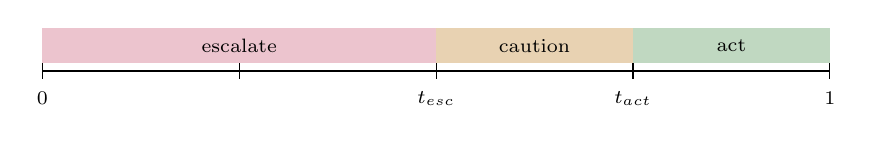
\begin{tikzpicture}[every node/.style={font=\scriptsize}]
  \draw[thick] (0,0) -- (10,0);
  \foreach \x in {0,2.5,5,7.5,10} \draw (\x,0.1)--(\x,-0.1);
  \node at (0,-0.35){0}; \node at (5,-0.35){$t_{esc}$}; \node at (7.5,-0.35){$t_{act}$};
  \node at (10,-0.35){1};
  \fill[clSecurity!25] (0,0.1) rectangle (5,0.55);
  \fill[clInfra!30] (5,0.1) rectangle (7.5,0.55);
  \fill[clBackend!30] (7.5,0.1) rectangle (10,0.55);
  \node at (2.5,0.32){escalate}; \node at (6.25,0.32){caution}; \node at (8.75,0.32){act};
\end{tikzpicture}
\caption{The policy maps the gating statistic to three bands. Thresholds $t_{esc}, t_{act}$
are fitted per DP, primitive, and model version.\datalabel{Illustrative (docs/ARCHITECTURE.md \S6)}}
\label{fig:bands}
\end{figure}

\section{Security boundary}

Models advise; code authorizes. Untrusted inputs (user text, tool outputs) reach an advisory
layer (the LLM proposal, DP3/DP5 screens), but the authoritative layer (permission filter,
allow/deny lists, schema validation, human approval, sandbox) is deterministic. DP3 output
can only \emph{raise} the required approval level, never lower it.

\begin{figure}[h]\centering
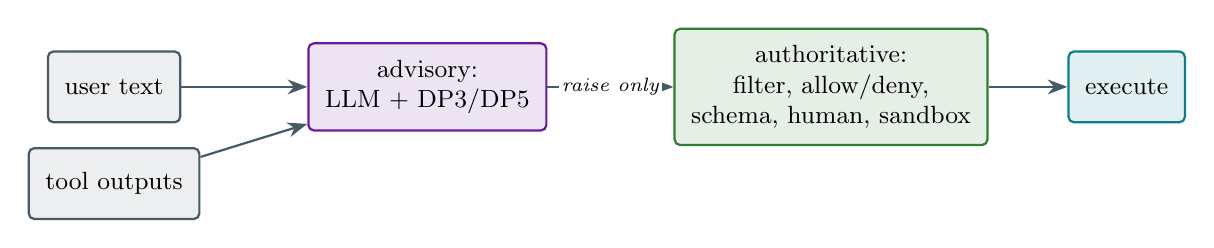
\begin{tikzpicture}[node distance=5mm and 10mm, every node/.style={font=\scriptsize}]
  \node[external] (u) {user text};
  \node[external, below=3mm of u] (o) {tool outputs};
  \node[model, right=16mm of u] (adv) {advisory:\\LLM + DP3/DP5};
  \node[backend, right=16mm of adv] (auth) {authoritative:\\filter, allow/deny,\\schema, human, sandbox};
  \node[frontend, right=of auth] (exec) {execute};
  \draw[flow] (u)--(adv); \draw[flow] (o)--(adv);
  \draw[flow] (adv)-- node[flowlabel]{raise only} (auth);
  \draw[flow] (auth)--(exec);
\end{tikzpicture}
\caption{Advisory vs authoritative layers. Injection is assumed; the engine is never the
boundary.\datalabel{Illustrative (docs/ARCHITECTURE.md \S10)}}
\label{fig:security}
\end{figure}

\section{Secrets: allow-list by reference}

The SDK never redacts secrets out of a model-visible string (a deny-list always misses
something). Instead, projections and logs carry secret \emph{names}; the executor injects
values at call time. A fuzz test smuggles a known token through every projection and asserts
it never appears.

\begin{lstlisting}[language=Python,caption={Engine swap is one line; the rest is unchanged.},label={lst:swap}]
dp2 = DecisionPoint(question=choice, engine=JevEngine(model="jev-1.13.0"), policy=policy)
# swap the engine, keep everything else:
dp2 = DecisionPoint(question=choice, engine=LLMAdapterEngine(provider="..."), policy=policy)
\end{lstlisting}

\begin{checkbox}
DP3 says a call is ``read-only'' with confidence 0.97, but the allow/deny list marks it
destructive. What happens, and which principle decides? (Appendix~\ref{app:answers}.)
\end{checkbox}

\chapter{Engineering practices}
\label{ch:engineering}

The SDK's credibility depends on boring, rigorous engineering. These practices come straight
from the plan review's findings.

\section{Record / replay cache}

Every model call is cached, keyed by a content hash of the request. This gives deterministic
offline re-runs (``one command regenerates every table, no API calls'') and makes results
reproducible.

\begin{figure}[h]\centering
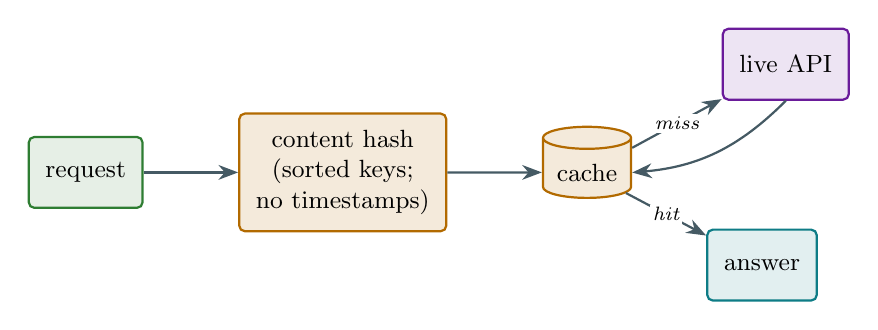
\begin{tikzpicture}[node distance=6mm and 12mm, every node/.style={font=\scriptsize}]
  \node[backend] (req) {request};
  \node[infra, right=of req] (hash) {content hash\\(sorted keys;\\no timestamps)};
  \node[store, right=of hash] (cache) {cache};
  \node[model, above right=4mm and 12mm of cache] (api) {live API};
  \node[frontend, below right=4mm and 12mm of cache] (ans) {answer};
  \draw[flow] (req)--(hash); \draw[flow] (hash)--(cache);
  \draw[flow] (cache)-- node[flowlabel]{miss} (api);
  \draw[flow] (api.south) to[bend left=20] (cache);
  \draw[flow] (cache)-- node[flowlabel]{hit} (ans);
\end{tikzpicture}
\caption{Record/replay: on a miss, call the API and store; on a hit, replay. The hash
excludes wall-clock and counters so it is stable across processes.\datalabel{Illustrative (docs/PLAN.md EF-11)}}
\label{fig:replay}
\end{figure}

\begin{pitfall}
Hash stability is easy to get wrong: Python's \texttt{PYTHONHASHSEED}, dict/set ordering, and
float formatting can all perturb serialization. The fix is canonical serialization (sorted
keys, excluded volatile fields) plus a cross-process test with a randomized hash seed.
\end{pitfall}

\section{Version pinning}

Every request pins an explicit Jev version and asserts the returned \texttt{model} field.
The alias \texttt{jev-latest} was observed re-pointing mid-run, and thresholds are
version-specific, so a version change must hard-fail and quarantine the run rather than
silently gate on stale calibrators.

\section{The test pyramid}

\begin{figure}[h]\centering
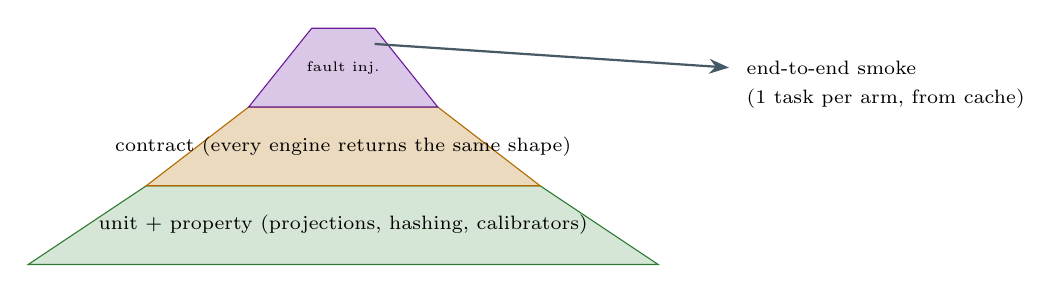
\begin{tikzpicture}[every node/.style={font=\scriptsize}]
  \fill[clBackend!20,draw=clBackend] (0,0)--(8,0)--(6.5,1)--(1.5,1)--cycle;
  \node at (4,0.5){unit + property (projections, hashing, calibrators)};
  \fill[clInfra!25,draw=clInfra] (1.5,1)--(6.5,1)--(5.2,2)--(2.8,2)--cycle;
  \node at (4,1.5){contract (every engine returns the same shape)};
  \fill[clModel!25,draw=clModel] (2.8,2)--(5.2,2)--(4.4,3)--(3.6,3)--cycle;
  \node[font=\tiny] at (4,2.5){fault inj.};
  \node[anchor=west,font=\scriptsize] at (9,2.5) {end-to-end smoke};
  \node[anchor=west,font=\scriptsize] at (9,2.1) {(1 task per arm, from cache)};
  \draw[flow] (4.4,2.8) -- (8.9,2.5);
\end{tikzpicture}
\caption{The test pyramid for the harness. Contract tests keep engines interchangeable;
fault injection proves the fallback path.\datalabel{Illustrative (docs/PLAN.md \S7.3)}}
\label{fig:pyramid}
\end{figure}

Specific tests the plan requires:
\begin{itemize}[itemsep=1pt]
  \item \textbf{Contract:} every engine returns the same typed shape; ``confidence
    unavailable'' is a first-class return (the LLM-adapter has no logprobs).
  \item \textbf{Property:} token budget never exceeded; projection output deterministic; no
    secret ever appears in a projection or log.
  \item \textbf{Fault injection:} fallback fires on 429/529/timeout, malformed JSON, and
    out-of-range Choice indices; the fallback reconstructs \emph{full} context so it is not
    handicapped by the lossy projection.
  \item \textbf{Fail-closed:} a state-machine test proves no side-effecting call reaches
    execution without the deterministic gate, and DP outputs may only feed
    narrow/deny/escalate, never allow/elevate.
  \item \textbf{Drift guard:} an injected distribution shift must trigger a fail-safe that
    widens bands or escalates.
\end{itemize}

\begin{whyhere}
Two subtle correctness traps the reviewer caught: (1) if the fallback feeds the LLM the
\emph{lossy} projection while the baseline sees full context, a fallback-heavy run looks
worse for reasons unrelated to the engine, biasing the whole evaluation; (2) the ``cost per
successful task'' denominator (``decision-equivalent tokens'') must be defined and
pre-registered, or the headline economic claim is unfalsifiable.
\end{whyhere}

\begin{checkbox}
Why must the fallback path rebuild full context instead of reusing the projection? What would
break in the evaluation if it did not? (Appendix~\ref{app:answers}.)
\end{checkbox}


\part{Evidence so far}
\chapter{Evidence so far}
\label{ch:evidence}

This chapter summarizes what independent testers found in the days after Jev's launch. All of
it is early, small, and unreproduced, so treat it as indicative, not settled. We have run no
experiments of our own yet, so there are no \MEAS{} labels here.

\section{Accuracy: competitive on short tasks, weak on long ones}

\begin{figure}[h]\centering
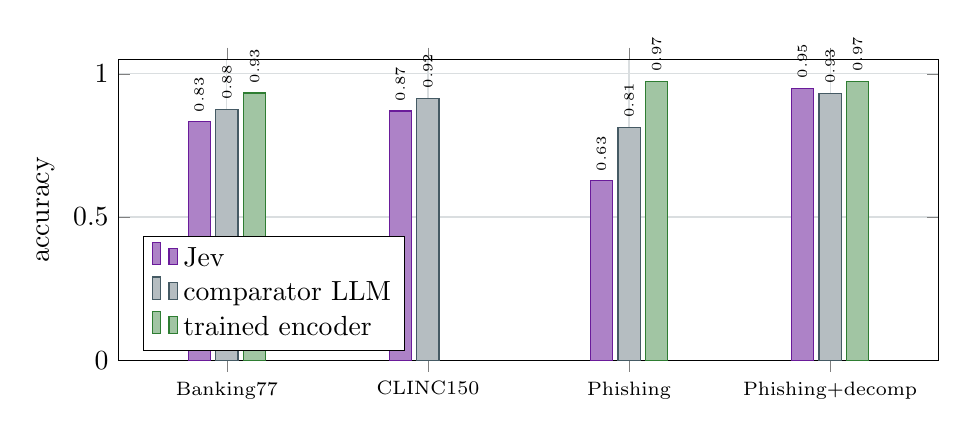
\begin{tikzpicture}
\begin{axis}[width=12cm,height=5.4cm,ybar,bar width=8pt,
  symbolic x coords={Banking77,CLINC150,Phishing,Phishing+decomp},
  xtick=data, x tick label style={font=\scriptsize},
  ylabel={accuracy}, ymin=0, ymax=1.05, legend pos=south west, legend cell align=left,
  enlarge x limits=0.18, grid=both, grid style={clExternal!20},
  nodes near coords, every node near coord/.append style={font=\tiny, rotate=90, anchor=west}]
  \addplot[fill=clModel!55, draw=clModel] coordinates
    {(Banking77,0.832)(CLINC150,0.870)(Phishing,0.626)(Phishing+decomp,0.950)};
  \addlegendentry{Jev}
  \addplot[fill=clExternal!40, draw=clExternal] coordinates
    {(Banking77,0.875)(CLINC150,0.915)(Phishing,0.813)(Phishing+decomp,0.932)};
  \addlegendentry{comparator LLM}
  % Trained-encoder numbers exist only for Banking77 (bge-small+LR) and phishing (4B LoRA);
  % there is no published CLINC150 encoder figure, so that bar is deliberately omitted.
  \addplot[fill=clBackend!45, draw=clBackend] coordinates
    {(Banking77,0.933)(Phishing,0.974)(Phishing+decomp,0.974)};
  \addlegendentry{trained encoder}
\end{axis}
\end{tikzpicture}
\caption{Jev is within a few points of the comparator LLM on short-input intent
classification, clearly below on whole-document phishing, and recovers most of the gap when
the judgment is decomposed. The comparator is the frontier model GPT-5.6 Terra on
Banking77/CLINC150 and Claude Haiku 4.5 on phishing; the encoder is bge-small+logistic
regression on Banking77 and a 4B LoRA model on phishing (no published CLINC150 encoder
number, so that bar is omitted). A trained in-domain encoder tends to win when labels
exist.\datalabel{Reported by jev-baselines-eval and jev-phishing-bench}~\citep{jev_baselines_eval,jev_phishing_bench}}
\label{fig:accuracy}
\end{figure}

\section{Latency: fast, but with tails under load}

Independent medians cluster around 0.24--0.9\,s per call depending on location and
concurrency, with rare tails of tens of seconds at high concurrency~\citep{aman_kumar}. Fast
enough to ask every step; the tails are why the SDK must be complete without Jev.

\begin{figure}[h]\centering
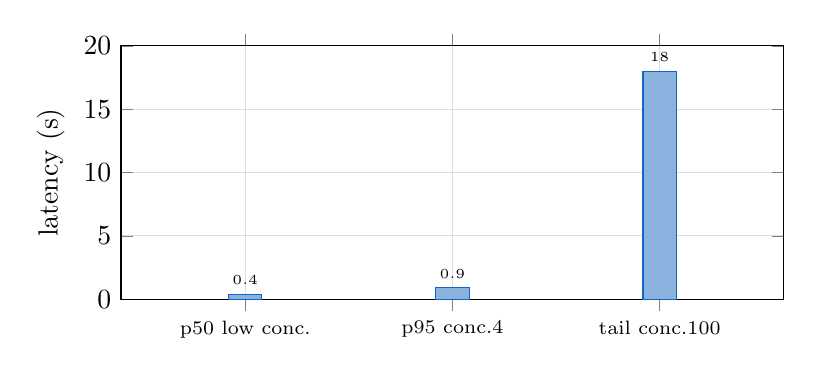
\begin{tikzpicture}
\begin{axis}[width=10cm,height=4.8cm,ybar,bar width=12pt,
  symbolic x coords={p50 low conc.,p95 conc.4,tail conc.100},
  xtick=data, x tick label style={font=\scriptsize},
  ylabel={latency (s)}, ymin=0, ymax=20, enlarge x limits=0.3,
  grid=both, grid style={clExternal!20}, nodes near coords,
  every node near coord/.append style={font=\tiny}]
  \addplot[fill=clAccent!50, draw=clAccent] coordinates
    {(p50 low conc.,0.4)(p95 conc.4,0.9)(tail conc.100,18)};
\end{axis}
\end{tikzpicture}
\caption{Illustrative latency profile: sub-second typical, multi-second tails under heavy
concurrency.\datalabel{Illustrative; ranges reported by Aman Kumar}~\citep{aman_kumar}}
\label{fig:latency}
\end{figure}

\section{Calibration}

The out-of-distribution ECE result (Figure~\ref{fig:ece}) is the single most important
calibration finding: near the noise floor in distribution, about 4.4\(\times\) the floor out
of distribution, and type-dependent (Choice/Score overconfident, Noul
underconfident)~\citep{jev_ood_calibration}. Recalibration with a few hundred labels brings
ECE back toward $0.01$~\citep{jev_calibration_anthus}.

\section{Where the hypotheses stand}

\begin{figure}[h]\centering
\small
\begin{tabular}{@{}clp{6.2cm}@{}}
\toprule
ID & Hypothesis (abridged) & Status \\
\midrule
H0 & separating decision from reasoning helps & partially supported, unproven end-to-end \\
H1 & Jev picks the right tool (DP2) cheaply & plausible, vendor-supported, unmeasured on real catalogs \\
H2 & inserting it lowers cost/task w/o hurting pass\^{}k & \textbf{open --- the MVP hypothesis} \\
H3 & Jev judges progress (DP4) & untested \\
H4 & probabilities gate well after recalibration & partially supported \\
H5 & the benefit is specific to Jev, not typed points & open; ARM-A2 exists to test it \\
\bottomrule
\end{tabular}
\caption{Hypothesis status at the start of the build. The gates G0/G1/G2 are designed to move
these.\datalabel{Reported by docs/DECISION\_LOG.md \S1}}
\label{fig:hypotheses}
\end{figure}

\begin{whyhere}
The honest expected outcome, from the whole evidence base, is ``cheaper decisions at equal or
slightly lower accuracy, useful after recalibration.'' The project is built so that this
result, if it holds, is a \emph{success}: it is exactly the controlled evidence nobody has
published, and the SDK ships it reproducibly.
\end{whyhere}

\begin{checkbox}
Which single hypothesis, if it failed at gate G2, would most change the product story, and why?
(Appendix~\ref{app:answers}.)
\end{checkbox}


\part{Build log}
\chapter{Build log}
\label{ch:buildlog}

New dated entries are appended here as tasks finish, so this book doubles as a project diary.

\section*{Entry 0 --- Research and planning (2026-09-20 to 2026-09-27)}

\textbf{2026-09-20.} Research phase completed: four documents produced (RESEARCH,
ARCHITECTURE, IMPLEMENTATION\_PLAN, DECISION\_LOG). Research gate: \emph{MODIFY}. Key
conclusions: Jev is fast and cheap on bounded closed-set judgments over compact state; its
accuracy sits at or slightly below cheap LLMs and below trained encoders on hard tasks; its
calibration is imperfect out of distribution but recalibratable; the missing thing is
controlled evidence, not another integration.

\textbf{2026-09-27.} Product phase began. Decisions recorded:
\begin{itemize}[itemsep=1pt]
  \item \textbf{D11} --- the product is an open-source Python SDK (supersedes the
    harness-only scope D1 and the ``defer a library'' decision D9; closes D8).
    The install name is set in D17.
  \item \textbf{D12} --- \texttt{docs/PLAN.md} is the operational source of truth.
  \item \textbf{D13} --- Python 3.12 via \texttt{uv}.
  \item \textbf{D14} --- this LaTeX book, built with Tectonic, with a tracked master PDF.
  \item \textbf{D16} --- the evidence artifact is elevated to a co-headline deliverable.
\end{itemize}

Work done this session:
\begin{itemize}[itemsep=1pt]
  \item Git repository initialized; the four research docs committed as a baseline.
  \item Office-hours design doc written and passed an independent 3-round spec review
    (7\,$\to$\,8\,$\to$\,8/10, converged).
  \item Plan review (CEO, Eng, DX) run with independent reviewers; Codex was unavailable
    (expired token), so this was subagent-only. Findings folded into \texttt{PLAN.md} as
    engineering findings EF-01--EF-17 and DX findings, plus a strategic ``User Challenge''
    (Q17) surfaced for the user: consider making the evidence/benchmark the headline.
  \item \texttt{docs/PLAN.md} written (16 sections) and \texttt{DECISION\_LOG.md} amended.
  \item This learning book created and built with Tectonic; master PDF generated.
\end{itemize}

\textbf{Not done this session (by design):} SDK code, API keys, experiments, publishing.
Those begin at milestone M0.6 onward and need the human touchpoints listed in
\texttt{PLAN.md} \S10.

\section*{Entry 1 --- Package name (2026-09-27)}

\textbf{2026-09-27.} Adopted the package name \texttt{arbiter} (ARBITER: Agent Runtime
for Bounded Inference, Triage, Evaluation \& Routing). Decision D17 supersedes the
working name in D15 and resolves Q16 for the install name. The import path is
\texttt{arbiter}. License and publishing stay at touchpoint H8.

\begin{keyidea}
The most important single artifact from the research phase is the ``jaggedness'' table
(Figure~\ref{fig:failuremodes}): nine documented failure modes that the entire architecture is
designed around.
\end{keyidea}


\appendix
\part{Appendices}
\chapter{Glossary}
\label{app:glossary}

\begin{description}[style=nextline,leftmargin=0.6cm]
  \item[Agent loop]\index{agent loop} observe, decide, act, observe again; the cycle an LLM
    agent runs.
  \item[ARBITER]\index{ARBITER} Agent Runtime for Bounded Inference, Triage, Evaluation \&
    Routing. The product. The Python package and import name is \texttt{arbiter} (D17).
  \item[AUROC]\index{AUROC} area under the ROC curve; here, how well a confidence score ranks
    correct answers above incorrect ones (0.5 = chance, 1.0 = perfect).
  \item[Brier score]\index{Brier score} mean squared error between predicted probabilities
    and outcomes; a proper scoring rule for probabilistic predictions.
  \item[Calibration]\index{calibration} the property that predictions stated at probability
    $p$ are correct a fraction $p$ of the time, measured over groups.
  \item[Cascade]\index{cascade} try a cheap model first, escalate to an expensive one on low
    confidence.
  \item[Choice]\index{Choice} a Jev primitive: pick one of up to 255 options; returns
    per-option probabilities and a confidence.
  \item[Confidence (Jev field)]\index{confidence} a statistic of the probability
    distribution; formula undisclosed; independently found weaker than max probability for
    gating.
  \item[Conformal prediction]\index{conformal prediction} builds a set guaranteed to contain
    the truth with chosen probability, using a calibration set.
  \item[Coverage]\index{coverage} the fraction of decisions a policy acts on automatically at
    a given threshold.
  \item[Decision point (DP)]\index{decision point} a bounded, closed-set decision in the
    agent loop (DP1--DP7).
  \item[ECE]\index{ECE} expected calibration error; average gap between confidence and
    accuracy across probability bins.
  \item[Engine]\index{engine} the swappable component that answers a decision question (Jev,
    LLM-adapter, classifier, rules, oracle, random).
  \item[Gate (G0/G1/G2)]\index{gate} a go/modify/stop checkpoint with pre-registered criteria.
  \item[Isotonic regression]\index{isotonic regression} a monotonic post-hoc recalibrator
    that maps stated probability to observed frequency.
  \item[Noul]\index{Noul} a Jev primitive: the probability that a statement is true; no
    separate confidence.
  \item[Noise floor]\index{noise floor} the small nonzero ECE a perfectly calibrated model
    shows on finite data.
  \item[pass@k / pass\^{}k]\index{passk@\texttt{pass\textasciicircum k}} success in at least
    one of $k$ tries / in all $k$ tries; the latter measures reliability.
  \item[Pareto frontier]\index{Pareto frontier} the set of systems not beaten on both cost
    and accuracy at once.
  \item[Policy table]\index{policy table} the deterministic rules mapping a gating statistic
    to act/narrow/escalate.
  \item[Projection]\index{projection} a token-budgeted, secret-free view of agent state sent
    to the engine.
  \item[Record/replay cache]\index{record/replay cache} content-hashed store of model
    responses enabling deterministic offline re-runs.
  \item[Router]\index{router} sends each query to the cheapest capable model, deciding before
    paying.
  \item[Score]\index{Score} a Jev primitive: a position on an ordered 2--10 level scale.
  \item[System One model]\index{System One model} TypeSafe's term for a fast, bounded-judgment
    model (after Kahneman's System 1); Jev is one.
  \item[Temperature scaling]\index{temperature scaling} a one-parameter post-hoc recalibrator
    on logits.
  \item[Trajectory-level calibration]\index{trajectory-level calibration} calibration measured
    across checkpoints of a whole run, not just per step.
\end{description}

\chapter{Formula sheet}
\label{app:formulas}

\section*{Calibration}

\textbf{Expected Calibration Error} (binned into $B$ bins, $n_b$ items in bin $b$, $N$ total):
\[
\mathrm{ECE} = \sum_{b=1}^{B} \frac{n_b}{N}\,\bigl|\,\mathrm{acc}(b) - \mathrm{conf}(b)\,\bigr|.
\]

\textbf{Brier score} (binary outcome $y_i\in\{0,1\}$, predicted probability $p_i$):
\[
\mathrm{BS} = \frac{1}{N}\sum_{i=1}^{N} (p_i - y_i)^2 .
\]

\textbf{Temperature scaling} (logits $z$, learned scalar $T>0$):
\[
\hat p = \mathrm{softmax}(z / T).
\]
$T>1$ softens an overconfident model; $T<1$ sharpens an underconfident one.

\section*{Reliability}

\textbf{pass@k} and \textbf{pass\^{}k} for per-attempt success probability $p$:
\[
\mathrm{pass@}k = 1 - (1-p)^k, \qquad \mathrm{pass\hat{}}k = p^{\,k}.
\]

\section*{Economics}

\textbf{Cost per successful task} (all model + fallback calls, in USD):
\[
\mathrm{CPST} = \frac{\text{total USD across all calls}}{\text{number of successful tasks}}.
\]

\textbf{Jev input cost} at list price (\$0.042 per million input tokens, output free):
\[
\mathrm{cost} = 0.042 \times \frac{\text{input tokens}}{10^6}\ \text{USD}.
\]

\section*{Worked examples}

\begin{worked}
For $p=0.7$ and $k=4$: $\mathrm{pass@}4 = 1-0.3^4 = 0.9919$, while
$\mathrm{pass\hat{}}4 = 0.7^4 = 0.2401$. The gap is why we report pass\^{}k
(Figure~\ref{fig:passk}).\datalabel{Exact (computed from formula)}
\end{worked}

\begin{worked}
20{,}000 decisions at 1{,}500 input tokens each:
$0.042 \times (20000 \times 1500)/10^6 = 0.042 \times 30 = \$1.26$.\datalabel{Exact (computed from list price)}
\end{worked}

\chapter{Answers to ``Check yourself''}
\label{app:answers}

\begin{enumerate}[leftmargin=1.1cm]
\answitem{\textbf{(Ch.~\ref{ch:building})} An answer can be right by luck or on easy items
  while the stated confidence does not track correctness across the distribution. You catch it
  by measuring calibration (a reliability diagram and ECE against the noise floor), not just
  accuracy.}
\answitem{\textbf{(Ch.~\ref{ch:roadmap})} The record/replay cache makes every result
  reproducible offline with no API calls, so at gate review you can regenerate every table and
  audit exactly what was measured. It also removes network flakiness and cost from the
  build-test loop.}
\answitem{\textbf{(Ch.~\ref{ch:agents})} Guaranteed: valid output shape and a valid schema for
  tool arguments. Not guaranteed: a probability distribution over which tool was chosen. The
  decision layer adds that calibrated probability.}
\answitem{\textbf{(Ch.~\ref{ch:jev})} (1) Adversarial content is a documented Jev weakness, so
  it can be fooled by a benign-looking wrapper. (2) A saturated confidence of 0.99 can be
  wrong, and safety-critical authorization must be deterministic; code and allow/deny lists,
  not a probability, decide.}
\answitem{\textbf{(Ch.~\ref{ch:calibration})} 92\% accuracy with ECE 0.15 means the
  probabilities are badly miscalibrated, so ``confidence $\ge 0.9$'' may include many wrong
  items. Inspect the reliability diagram (Figure~\ref{fig:reliability}) and the ECE-vs-floor
  bars (Figure~\ref{fig:ece}) first, then recalibrate before gating.}
\answitem{\textbf{(Ch.~\ref{ch:routers})} Because Jev is so cheap it can be queried
  \emph{before} paying for the LLM, like a pre-generation router; a cascade instead pays the
  cheap model first and only then decides, which wastes the cheap call when it defers.}
\answitem{\textbf{(Ch.~\ref{ch:eval})} pass@8 counts a single lucky success out of eight,
  while pass\^{}8 requires success in all eight; an unreliable per-attempt rate (say 0.7)
  gives $0.7^8 \approx 0.058$. See Figure~\ref{fig:passk}.}
\answitem{\textbf{(Ch.~\ref{ch:decisionpoints})} DP2 narrows because Jev cannot write tool
  arguments (no generation) and its choice is advisory; keeping the LLM in the loop preserves
  correctness. DP4 never declares success alone because ``done'' is safety-relevant and must
  be confirmed by a deterministic completion verifier.}
\answitem{\textbf{(Ch.~\ref{ch:arch})} The call is treated as destructive (most conservative
  wins); DP3 output can only raise the required approval level, never lower it. The principle
  is ``the engine advises, code authorizes.''}
\answitem{\textbf{(Ch.~\ref{ch:engineering})} If the fallback reused the lossy projection while
  the baseline saw full context, fallback-heavy runs would look worse for reasons unrelated to
  the engine, biasing the whole cost/quality comparison. Rebuilding full context keeps the
  arms comparable.}
\answitem{\textbf{(Ch.~\ref{ch:evidence})} H5: if ARM-A2 (an LLM answering the same typed
  questions) matches ARM-A1, the benefit is from typed decision points, not Jev specifically,
  so the product story shifts from ``Jev'' to ``calibrated typed decisions, with Jev as the
  cheap option.''}
\end{enumerate}

\chapter{Source map}
\label{app:sourcemap}

Where each chapter's material comes from in the frozen research docs and the operational
plan. Use this to trace any claim back to its origin.

\begin{longtable}{@{}p{5.2cm}p{7.0cm}@{}}
\toprule
Book chapter & Primary sources \\
\midrule
\endhead
Ch.~\ref{ch:building} What we are building & docs/PLAN.md \S2; design doc; RESEARCH \S5.5, \S10 \\
Ch.~\ref{ch:roadmap} The roadmap & docs/PLAN.md \S6--7; IMPLEMENTATION\_PLAN \S2--3 \\
Ch.~\ref{ch:agents} LLM agents & RESEARCH \S5.1; ARCHITECTURE \S1 \\
Ch.~\ref{ch:jev} Jev / System One & RESEARCH \S1, \S4; TypeSafe docs (models, primitives, jaggedness) \\
Ch.~\ref{ch:calibration} Calibration & RESEARCH \S4.3; jev-ood-calibration; Jev-Calibration; Guo et al. \\
Ch.~\ref{ch:routers} Routers/cascades & RESEARCH \S5.2; RouteLLM; FrugalGPT; cascade-deferral \\
Ch.~\ref{ch:eval} Evaluating agents & RESEARCH \S9; tau-bench; AI Agents That Matter \\
Ch.~\ref{ch:decisionpoints} Decision points & ARCHITECTURE \S3 \\
Ch.~\ref{ch:arch} SDK architecture & ARCHITECTURE \S4--10; docs/PLAN.md \S4--5, \S7.4 \\
Ch.~\ref{ch:engineering} Engineering practices & docs/PLAN.md \S7.3 (EF-01..EF-17); ARCHITECTURE \S9 \\
Ch.~\ref{ch:evidence} Evidence so far & RESEARCH \S4.2--4.3; independent studies (see bibliography) \\
Ch.~\ref{ch:buildlog} Build log & docs/DECISION\_LOG.md \S11; this session \\
\bottomrule
\end{longtable}

\begin{whyhere}
Data-quality note: RESEARCH.md lines 159--169 contain character-encoding corruption, and
three dollar figures there are unrecoverable. This book does not cite those three values;
they will be re-verified against the source cookbooks at task PT-2.1 before any use.
\end{whyhere}


\backmatter
\bibliographystyle{plainnat}
\bibliography{references}

\end{document}
